%!TEX root = ../thesis.tex
% ******************************* Thesis Appendix C ********************************

\chapter{}
\ifpdf
\graphicspath{{chapter-pmssm/Figs/Raster/}{chapter-pmssm/Figs/PDF/}{chapter-pmssm/Figs/}}
\else
\graphicspath{{chapter-pmssm/Figs/Vector/}{chapter-pmssm/Figs/}}
\fi

\section{Truth smearing}

\begin{figure}
	\centering
	\begin{subfigure}[b]{0.49\linewidth}
		\centering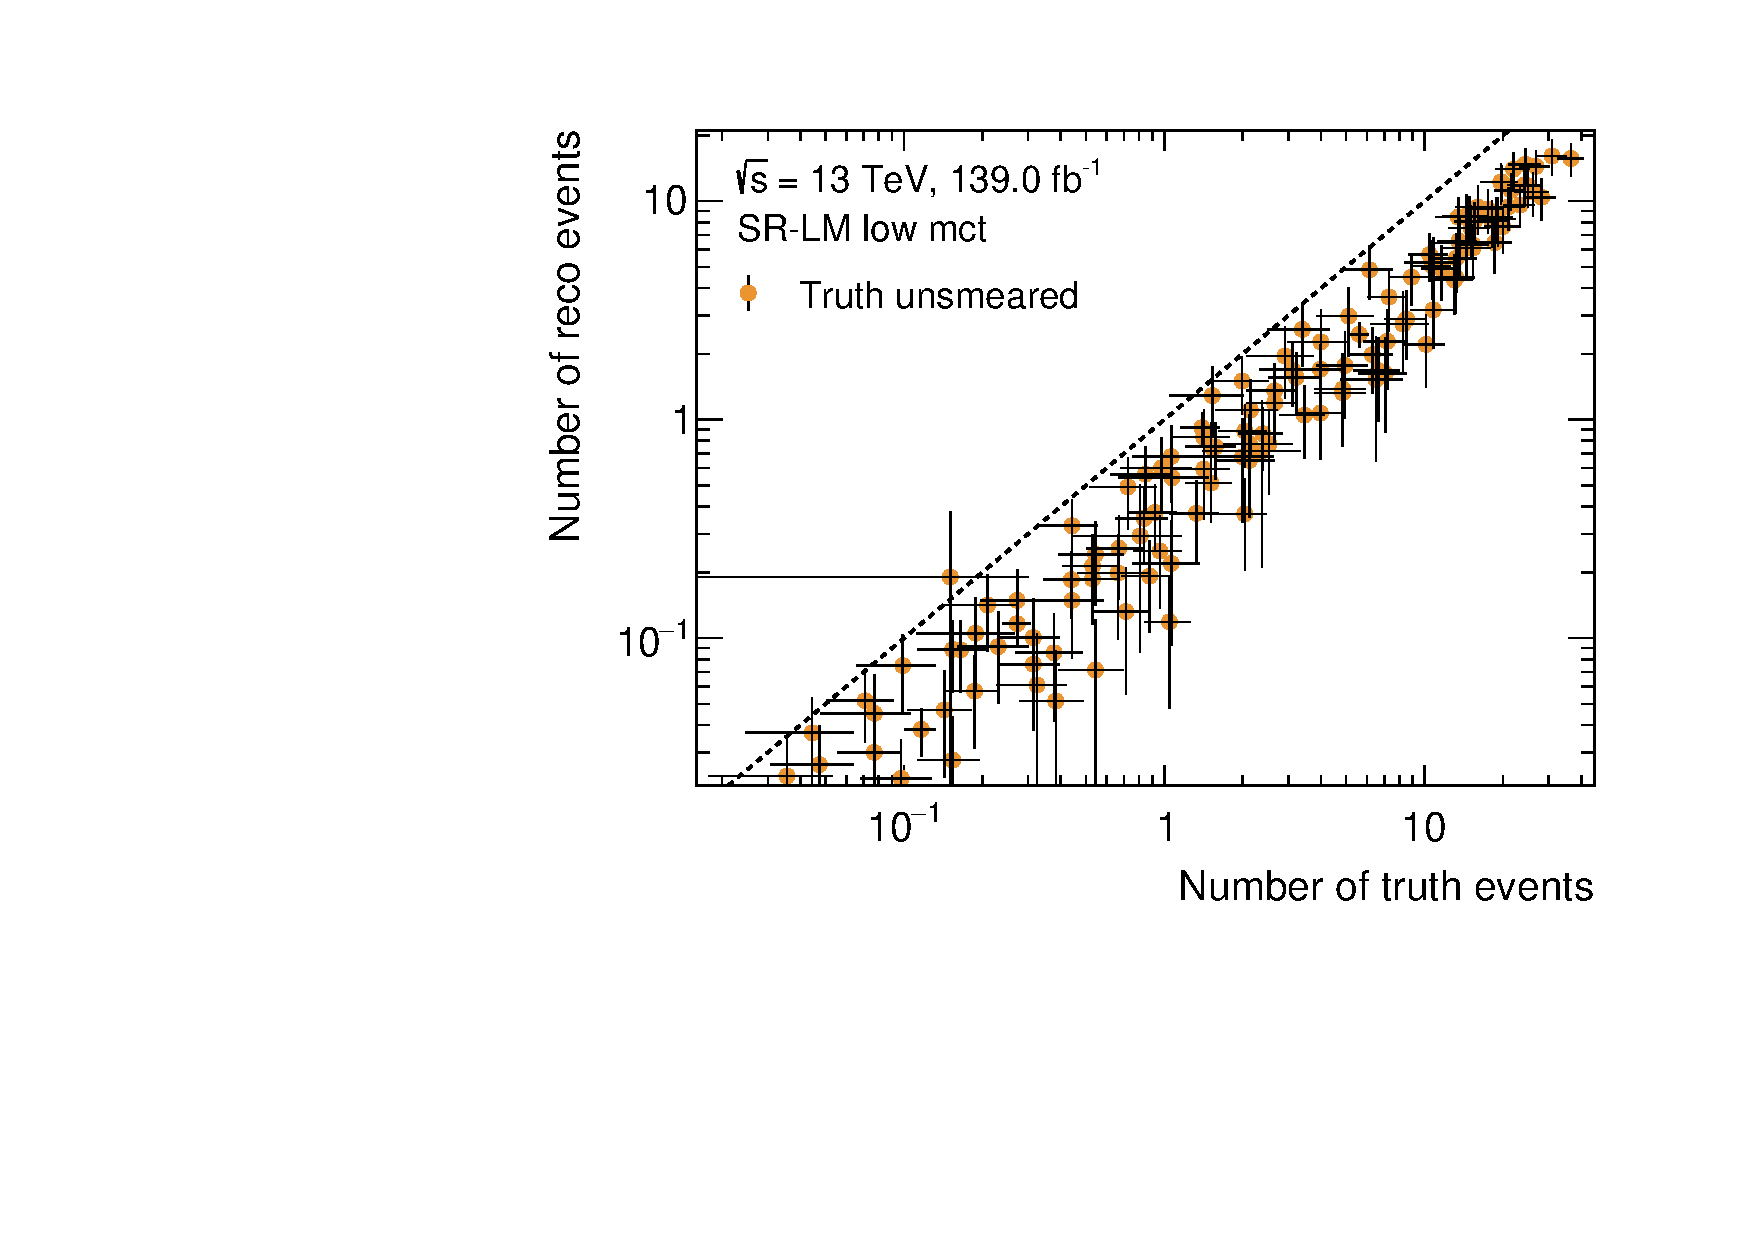
\includegraphics[width=\textwidth]{yields_SR-LM_low_mct_unsmeared}
	\end{subfigure}\hfill
	\begin{subfigure}[b]{0.49\linewidth}
		\centering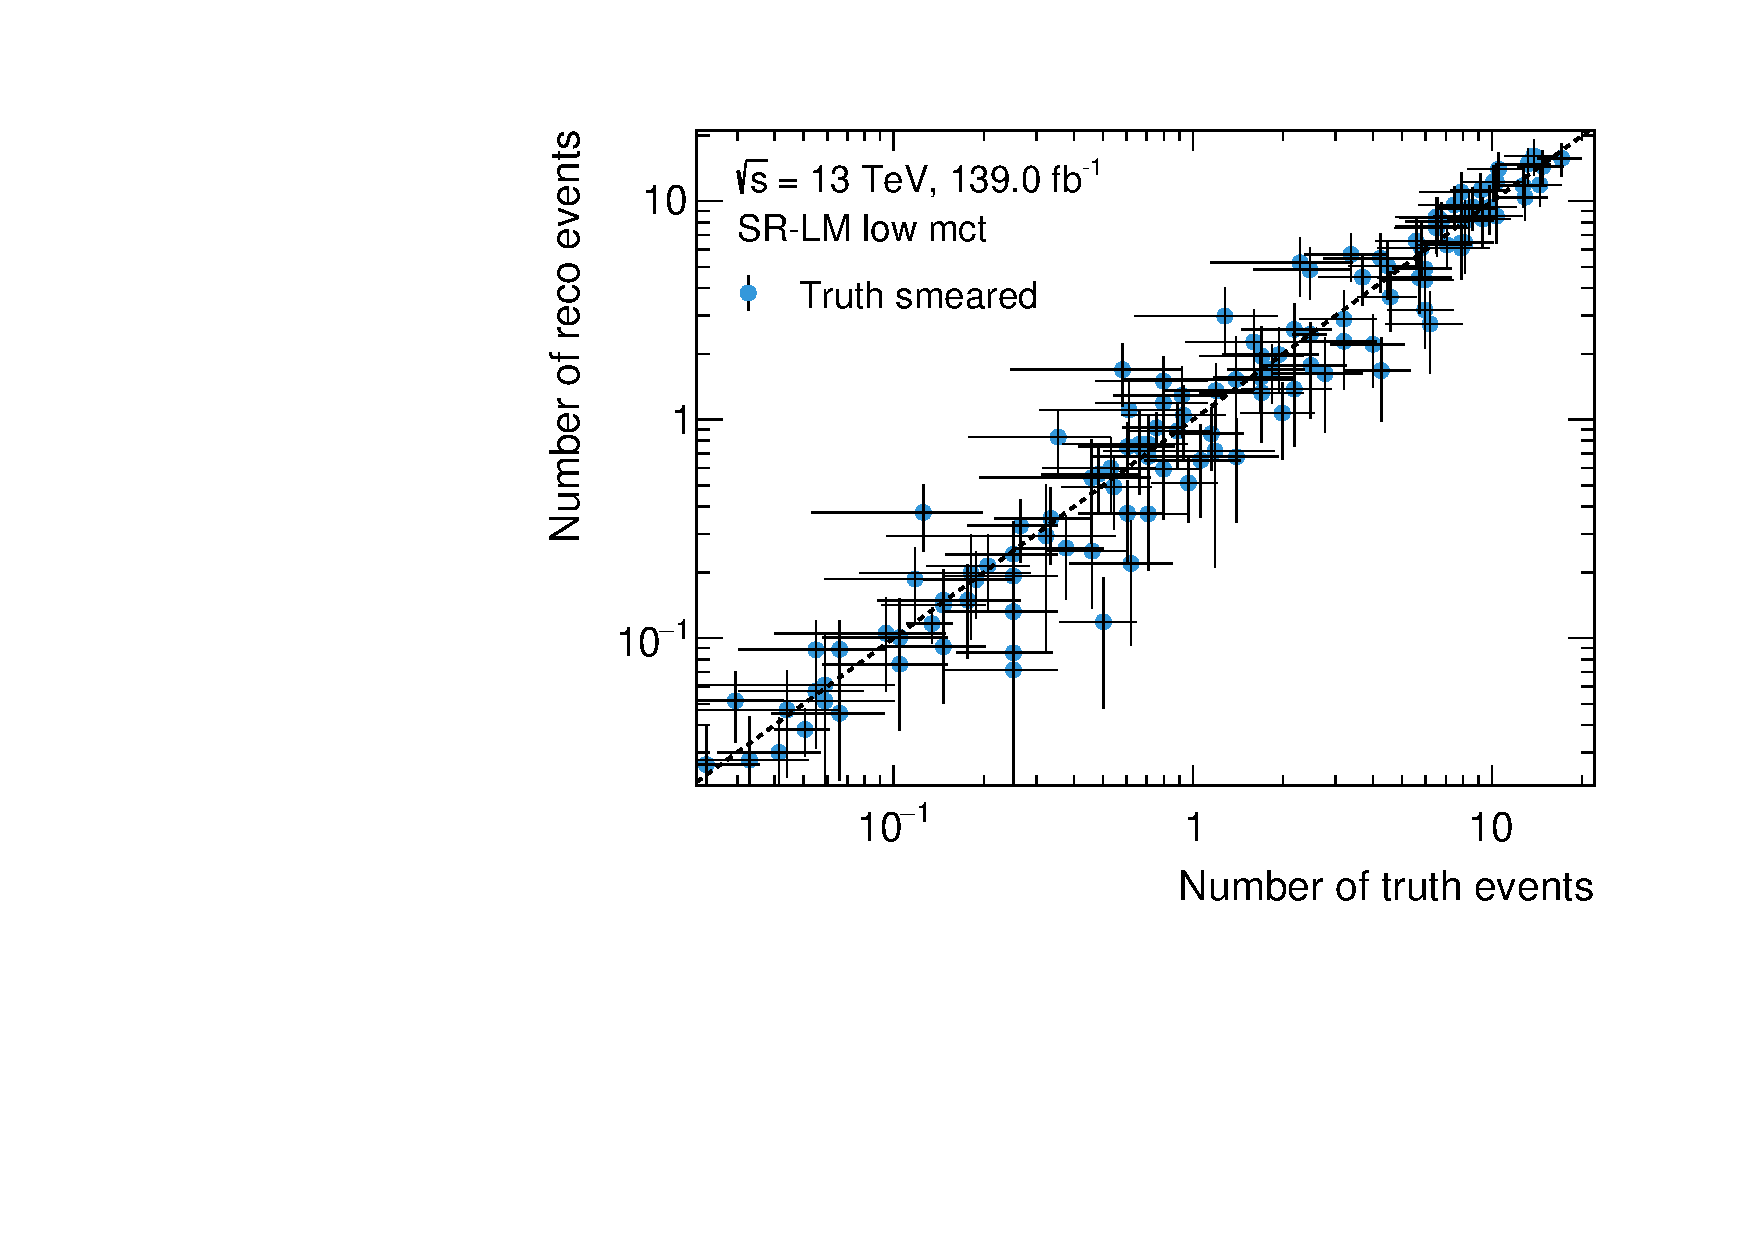
\includegraphics[width=\textwidth]{yields_SR-LM_low_mct_smeared}
	\end{subfigure}\hfill
	\begin{subfigure}[b]{0.49\linewidth}
		\centering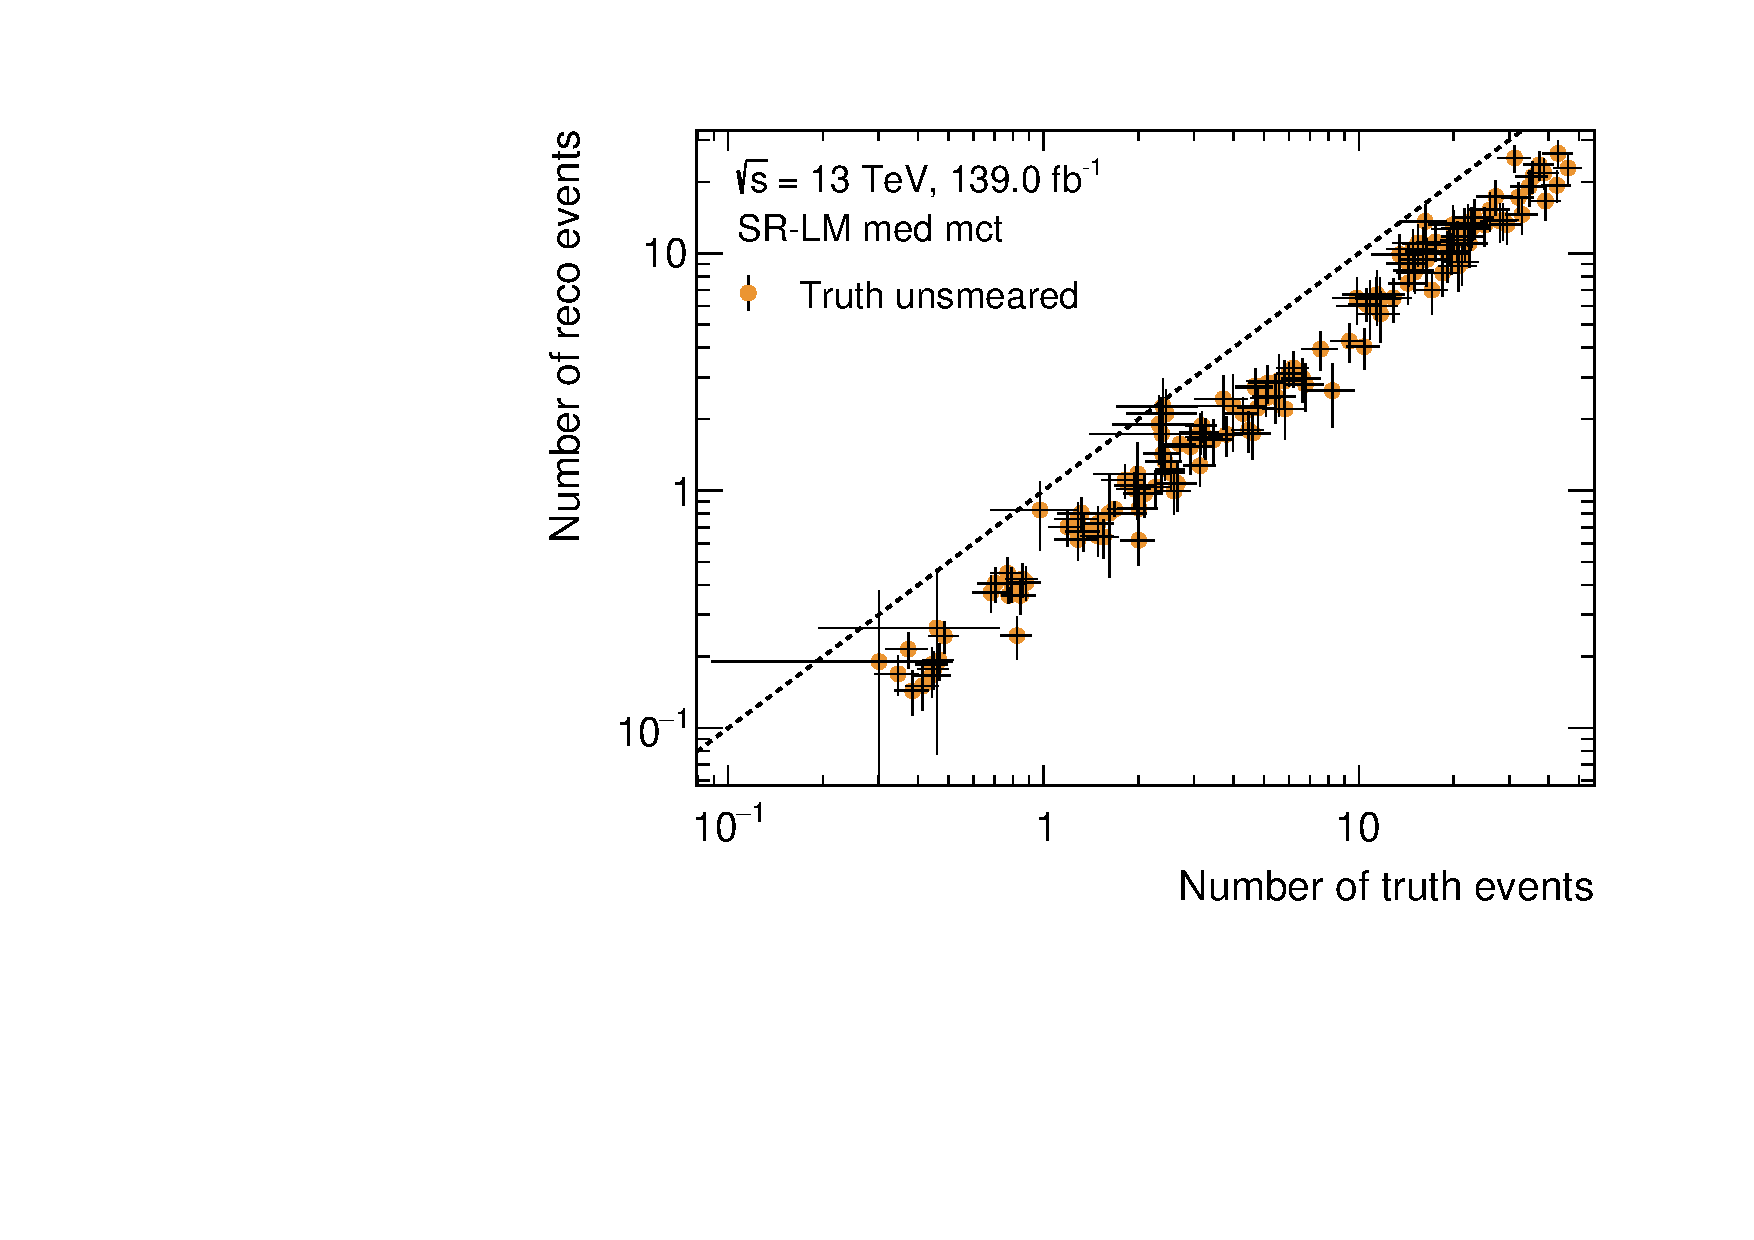
\includegraphics[width=\textwidth]{yields_SR-LM_med_mct_unsmeared}
	\end{subfigure}\hfill
	\begin{subfigure}[b]{0.49\linewidth}
		\centering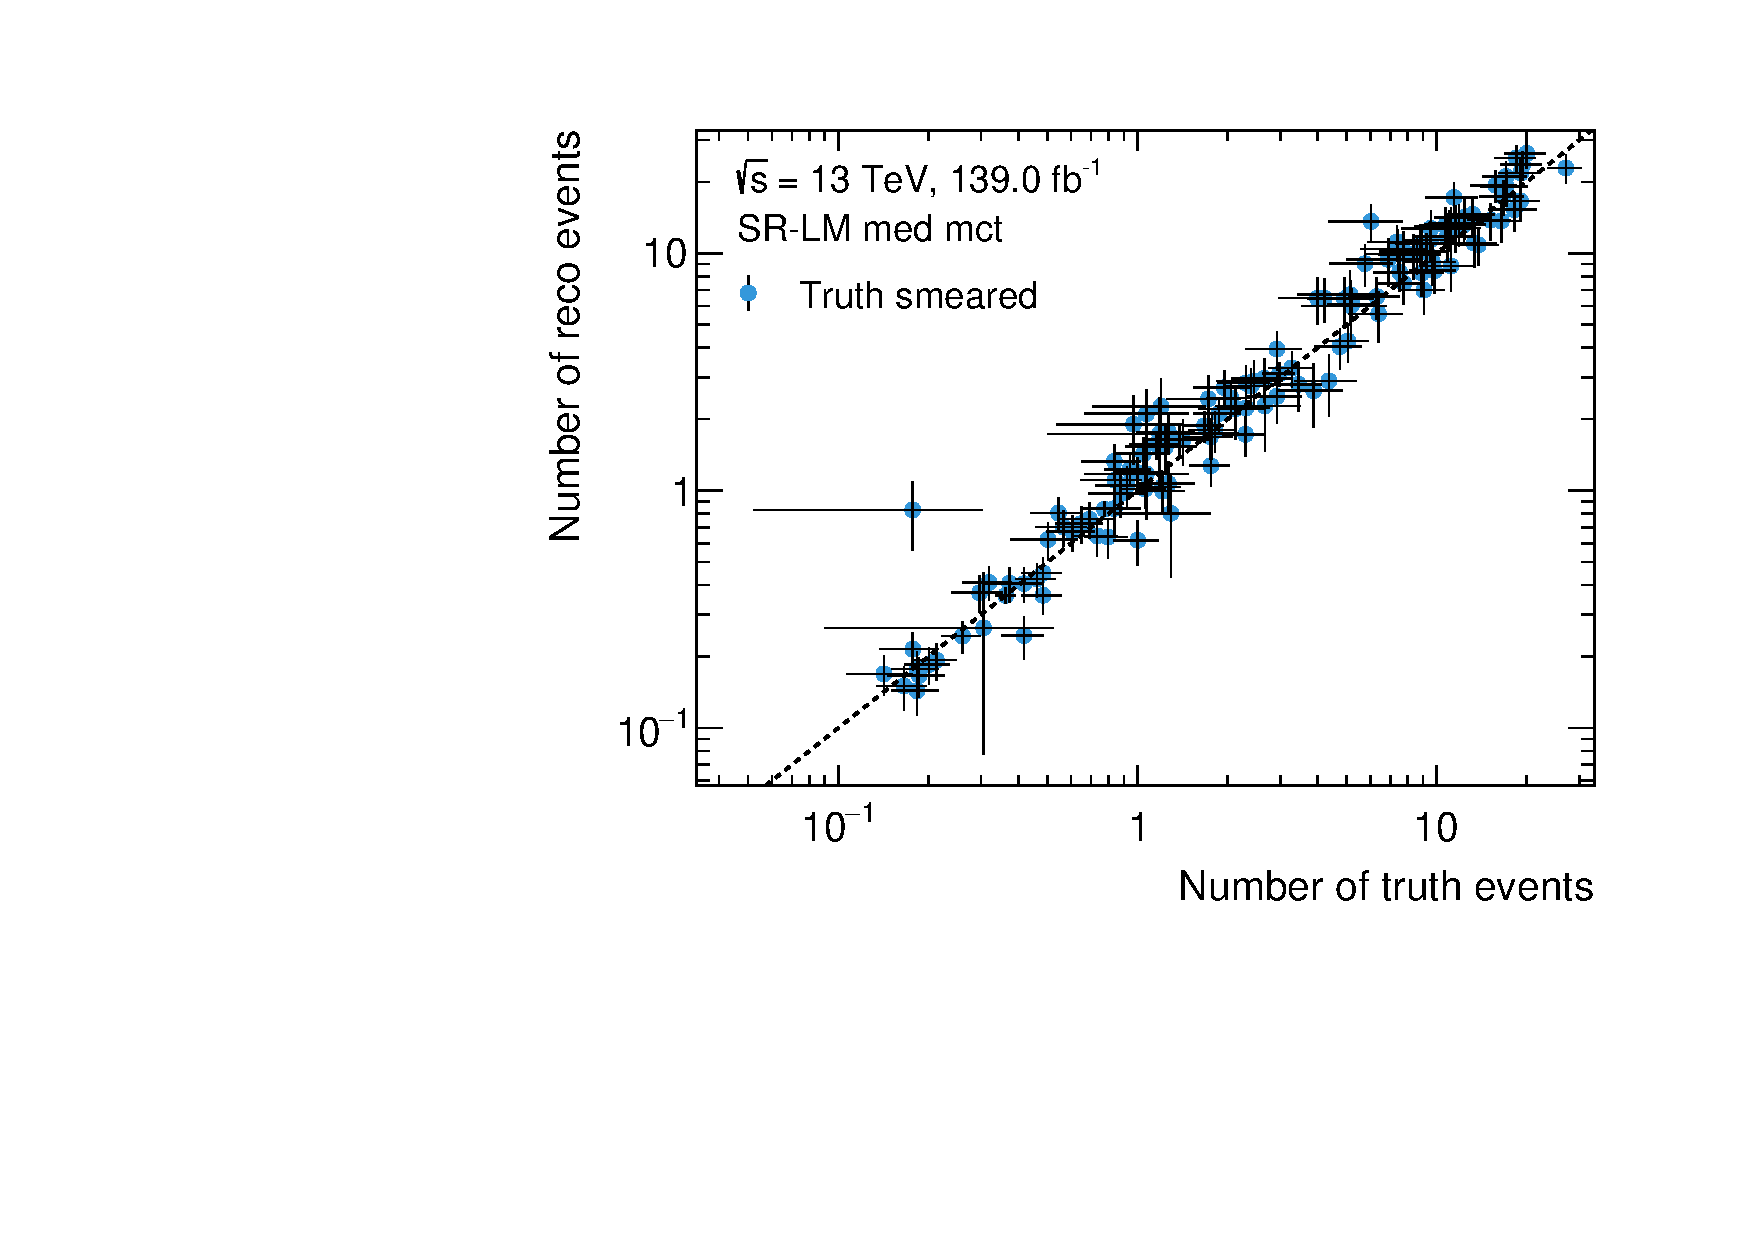
\includegraphics[width=\textwidth]{yields_SR-LM_med_mct_smeared}
	\end{subfigure}\hfill
	\begin{subfigure}[b]{0.49\linewidth}
		\centering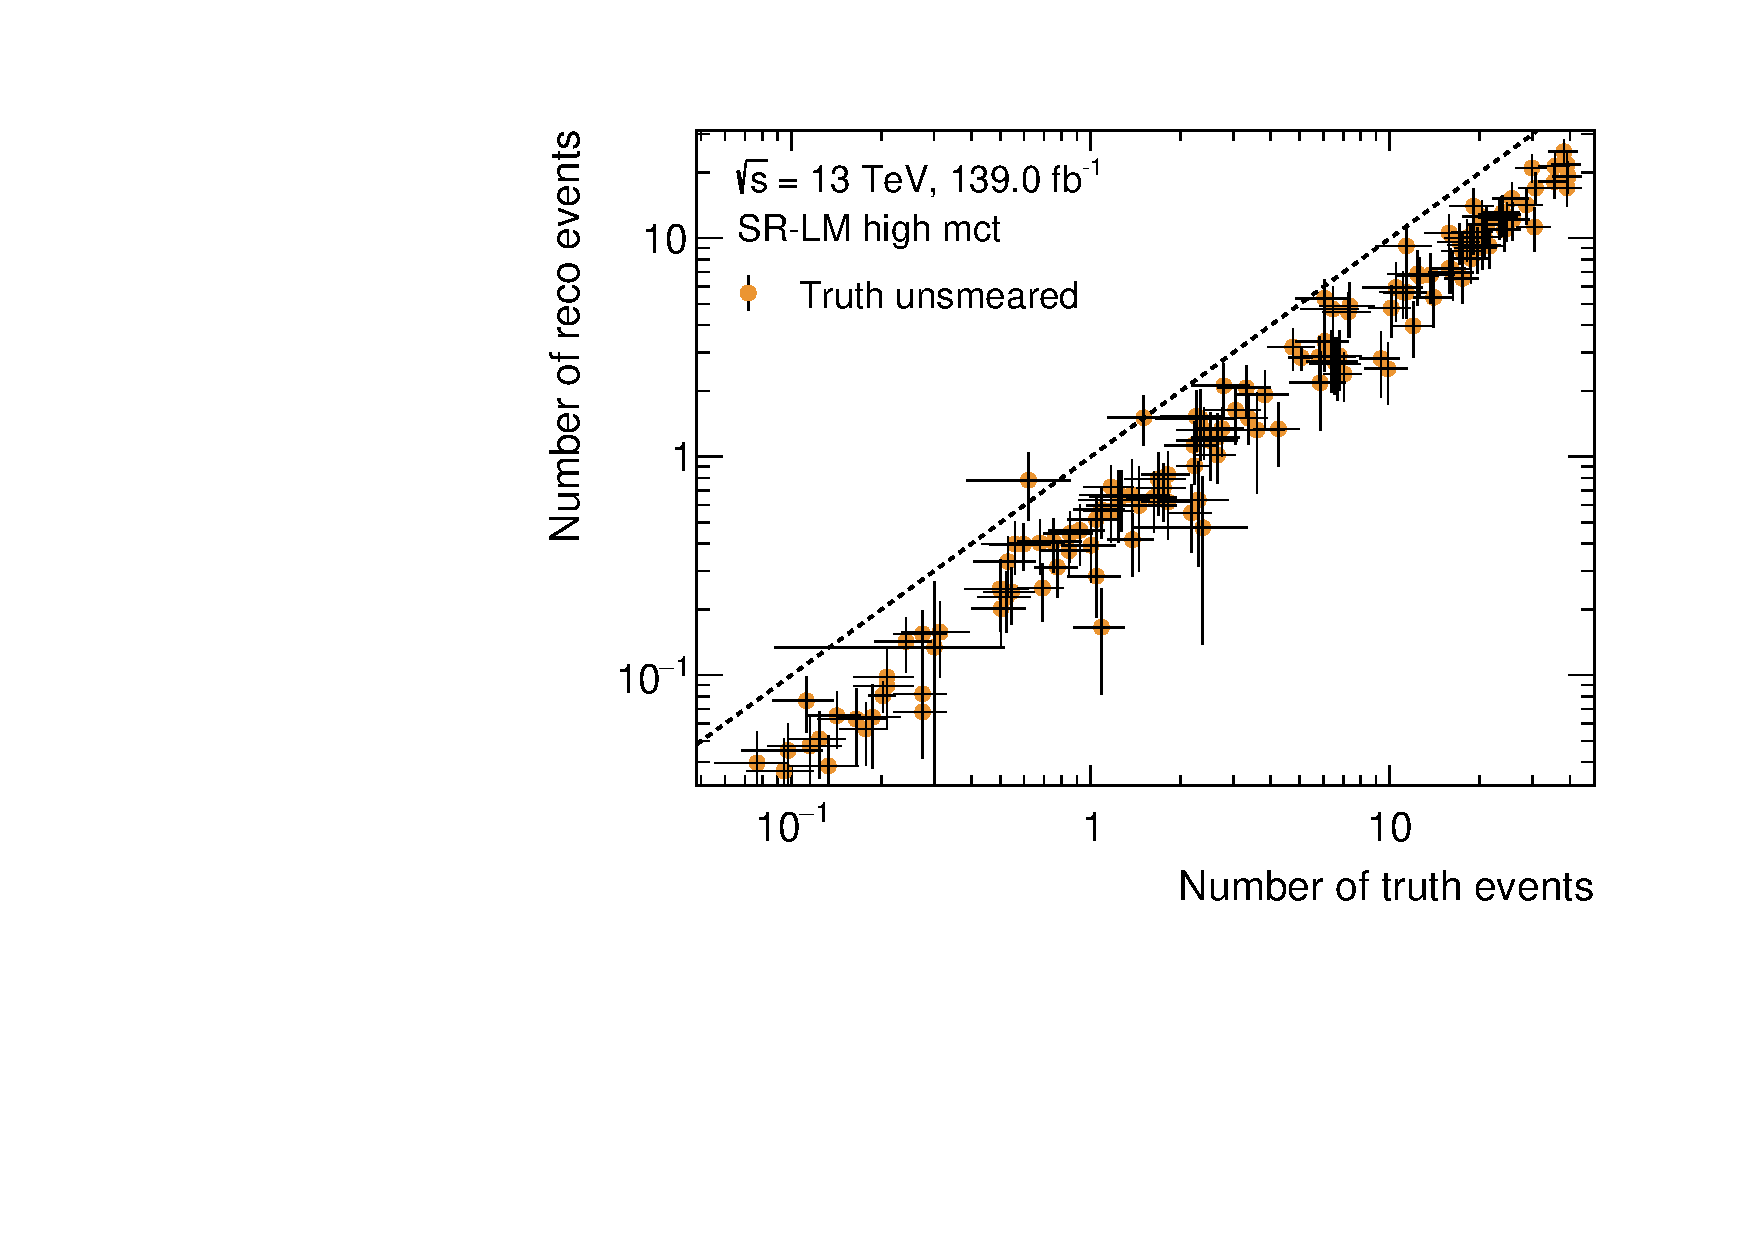
\includegraphics[width=\textwidth]{yields_SR-LM_high_mct_unsmeared}
	\end{subfigure}\hfill
	\begin{subfigure}[b]{0.49\linewidth}
		\centering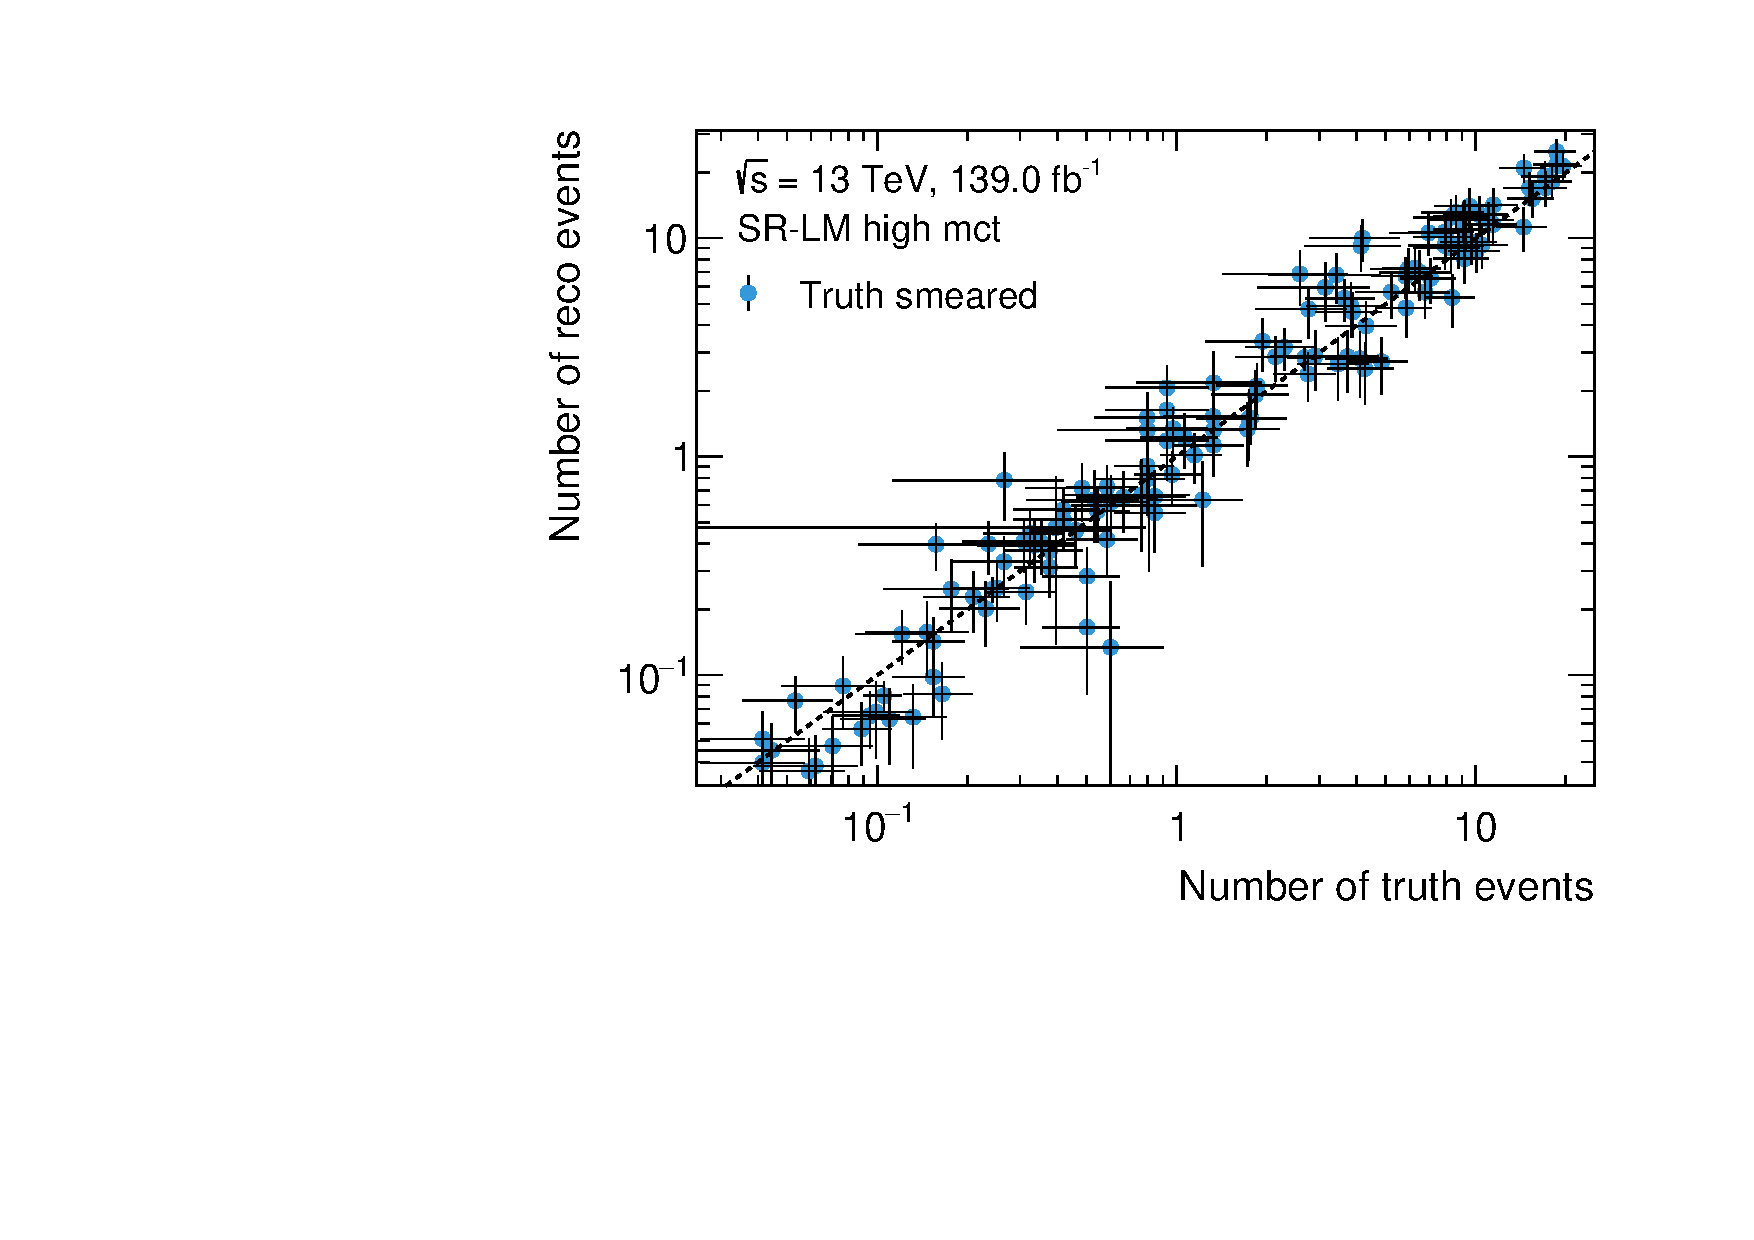
\includegraphics[width=\textwidth]{yields_SR-LM_high_mct_smeared}
	\end{subfigure}
	\caption{Comparison of the event rates at truth- and reconstruction-level before (left) and after (right) truth smearing in SR-LM. From top to bottom, the low, medium and high $\mct$ bins are shown. Every single point in the scatter plots represents a single signal model considered in the original 1-lepton analysis. Uncertainties include only \gls{mc} statistical uncertainties.}
	\label{fig:smearing_signal_regions_1}
\end{figure}

\begin{figure}
	\centering
	\begin{subfigure}[b]{0.49\linewidth}
		\centering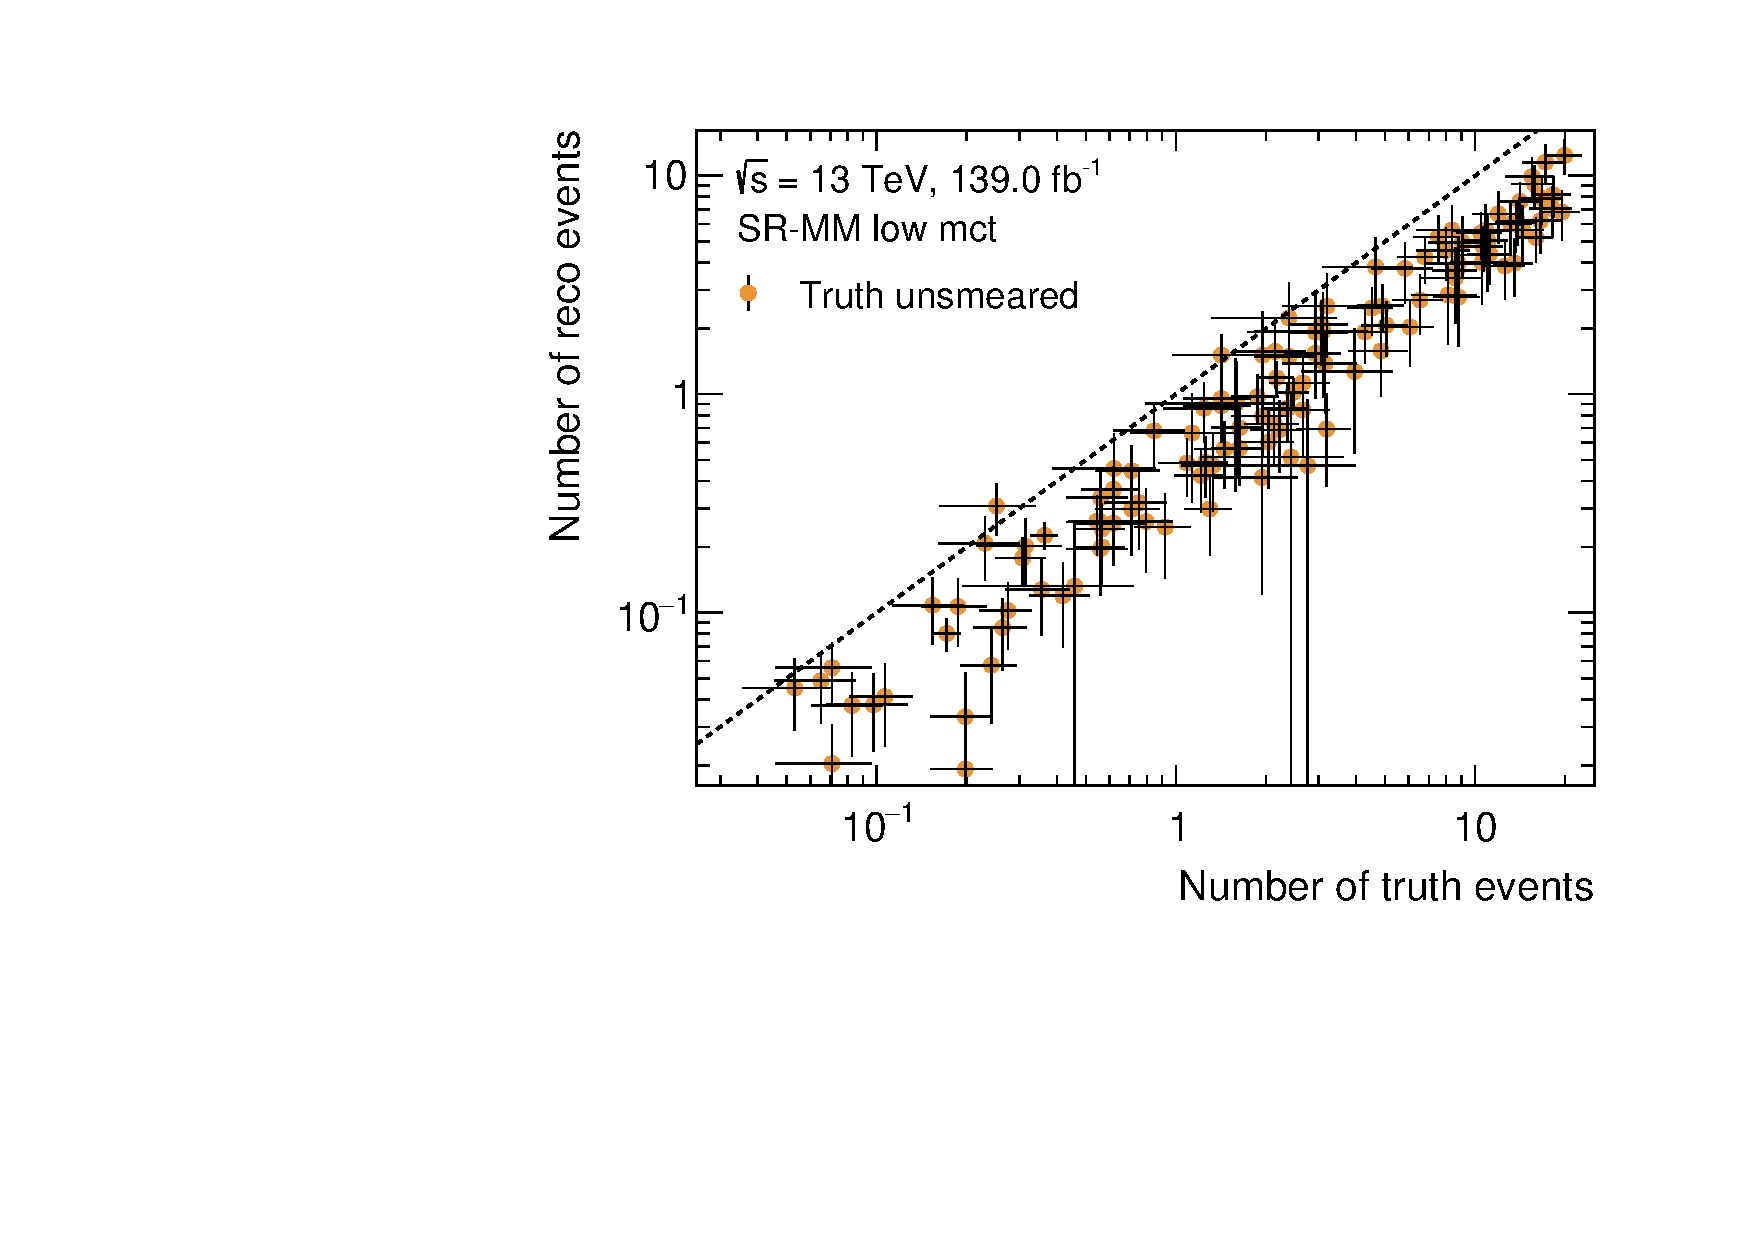
\includegraphics[width=\textwidth]{yields_SR-MM_low_mct_unsmeared}
	\end{subfigure}\hfill
	\begin{subfigure}[b]{0.49\linewidth}
		\centering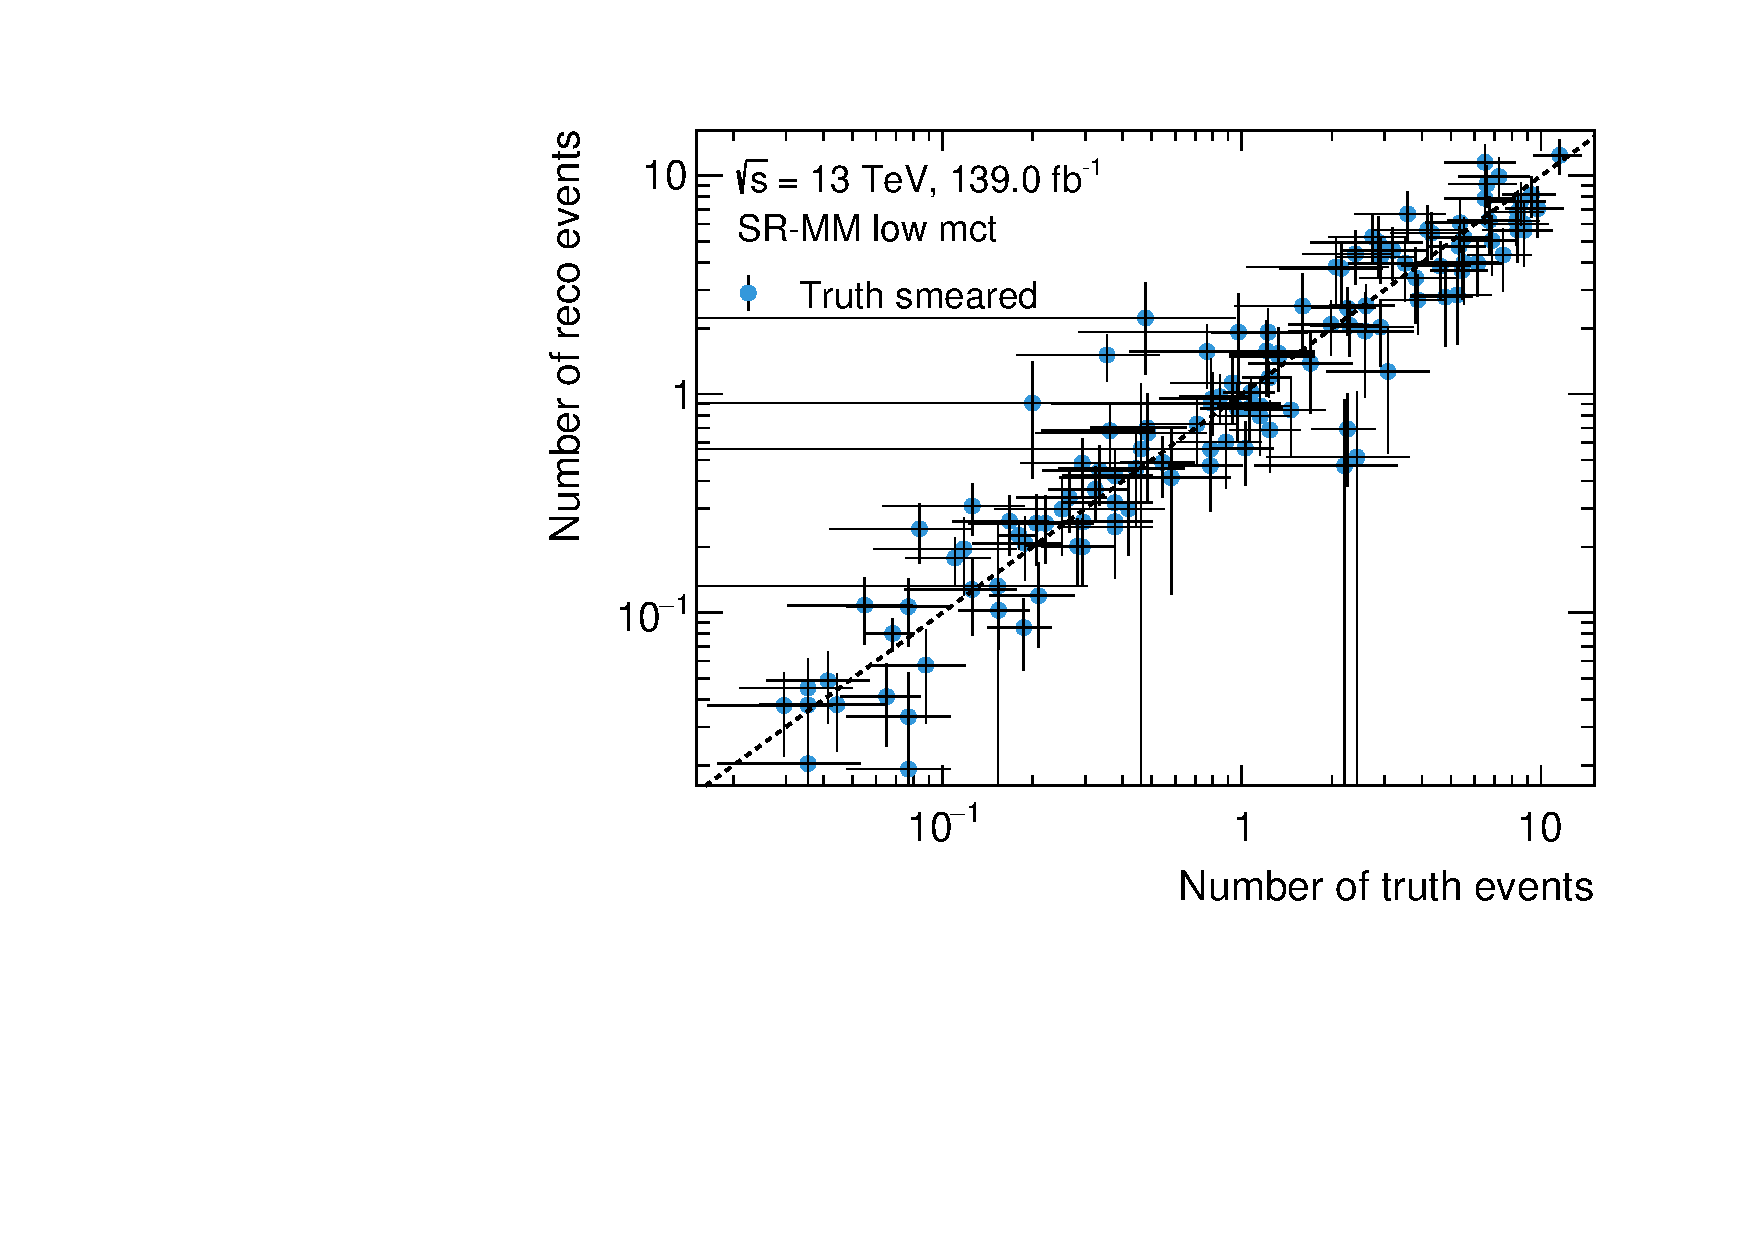
\includegraphics[width=\textwidth]{yields_SR-MM_low_mct_smeared}
	\end{subfigure}\hfill
	\begin{subfigure}[b]{0.49\linewidth}
		\centering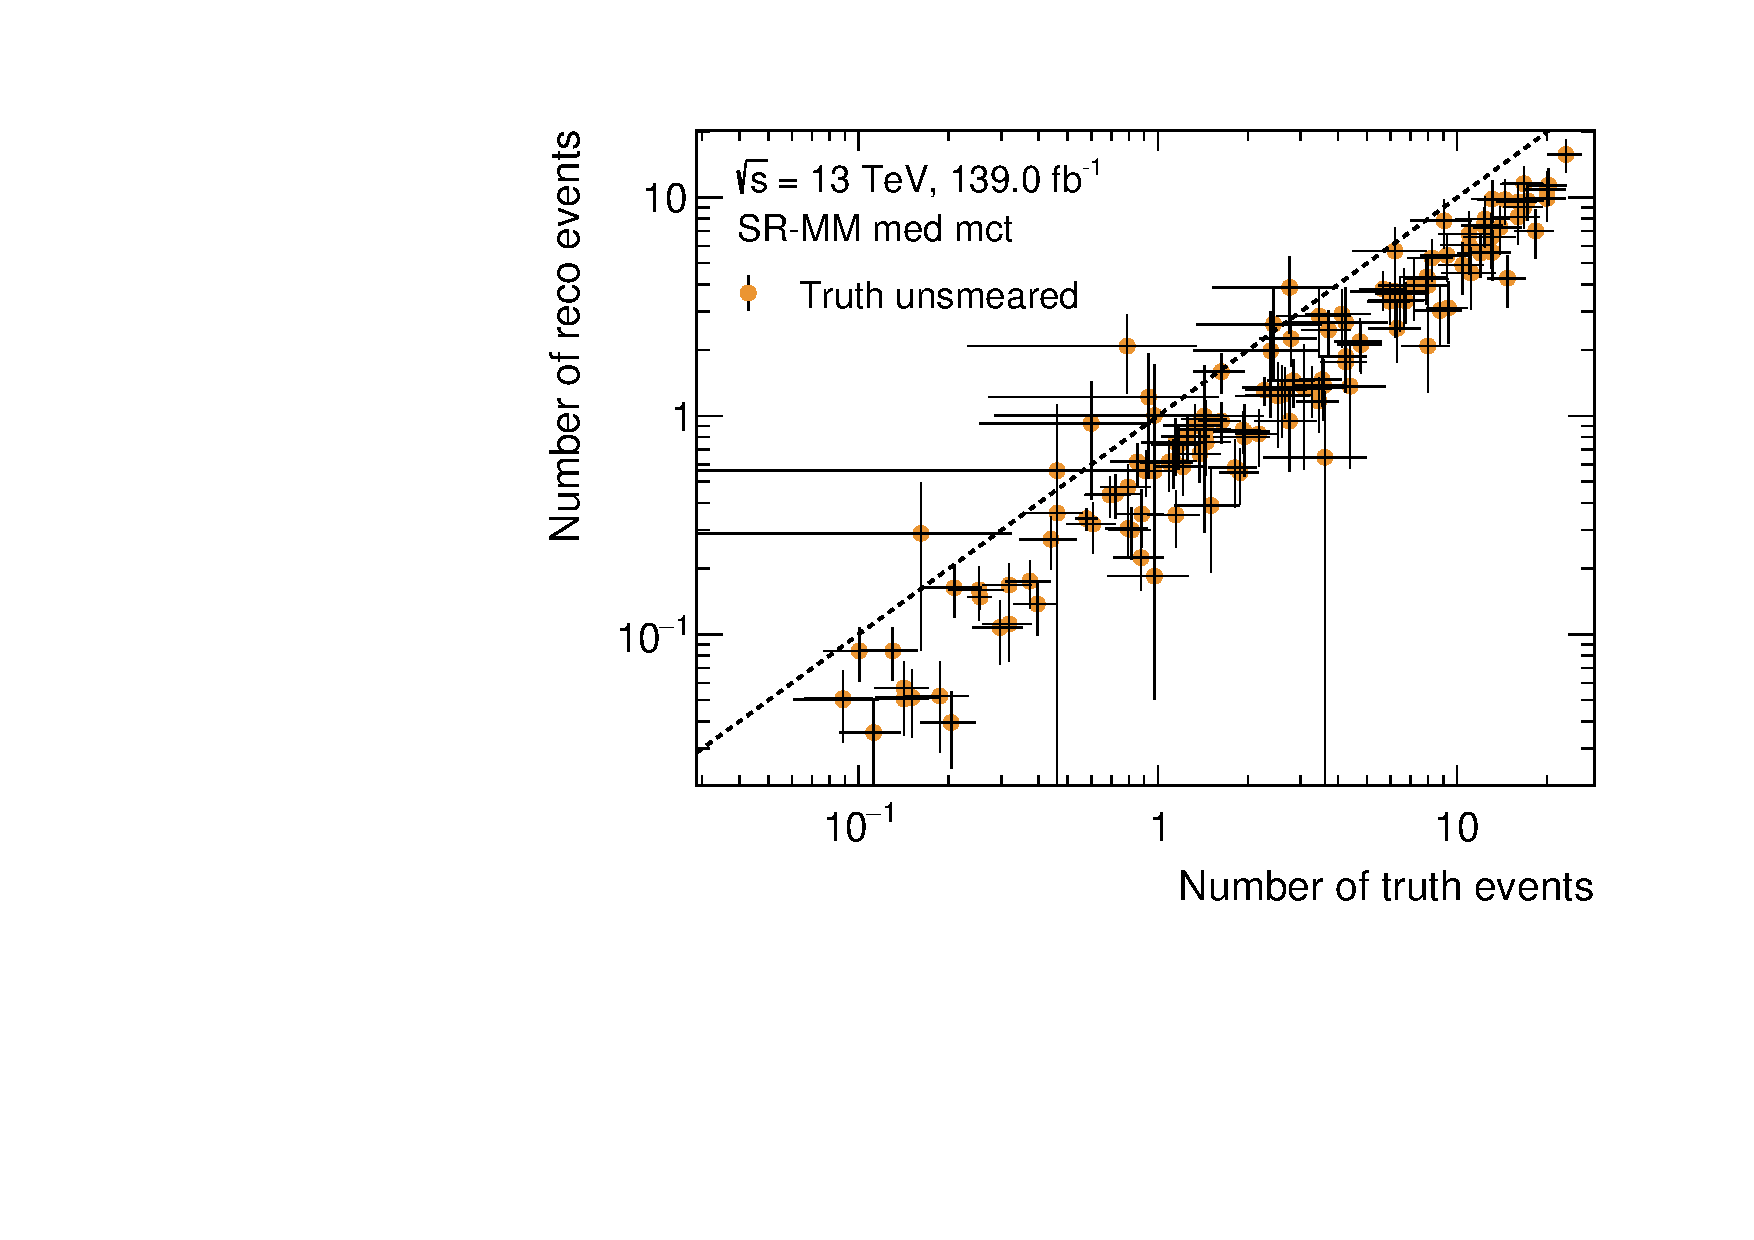
\includegraphics[width=\textwidth]{yields_SR-MM_med_mct_unsmeared}
	\end{subfigure}\hfill
	\begin{subfigure}[b]{0.49\linewidth}
		\centering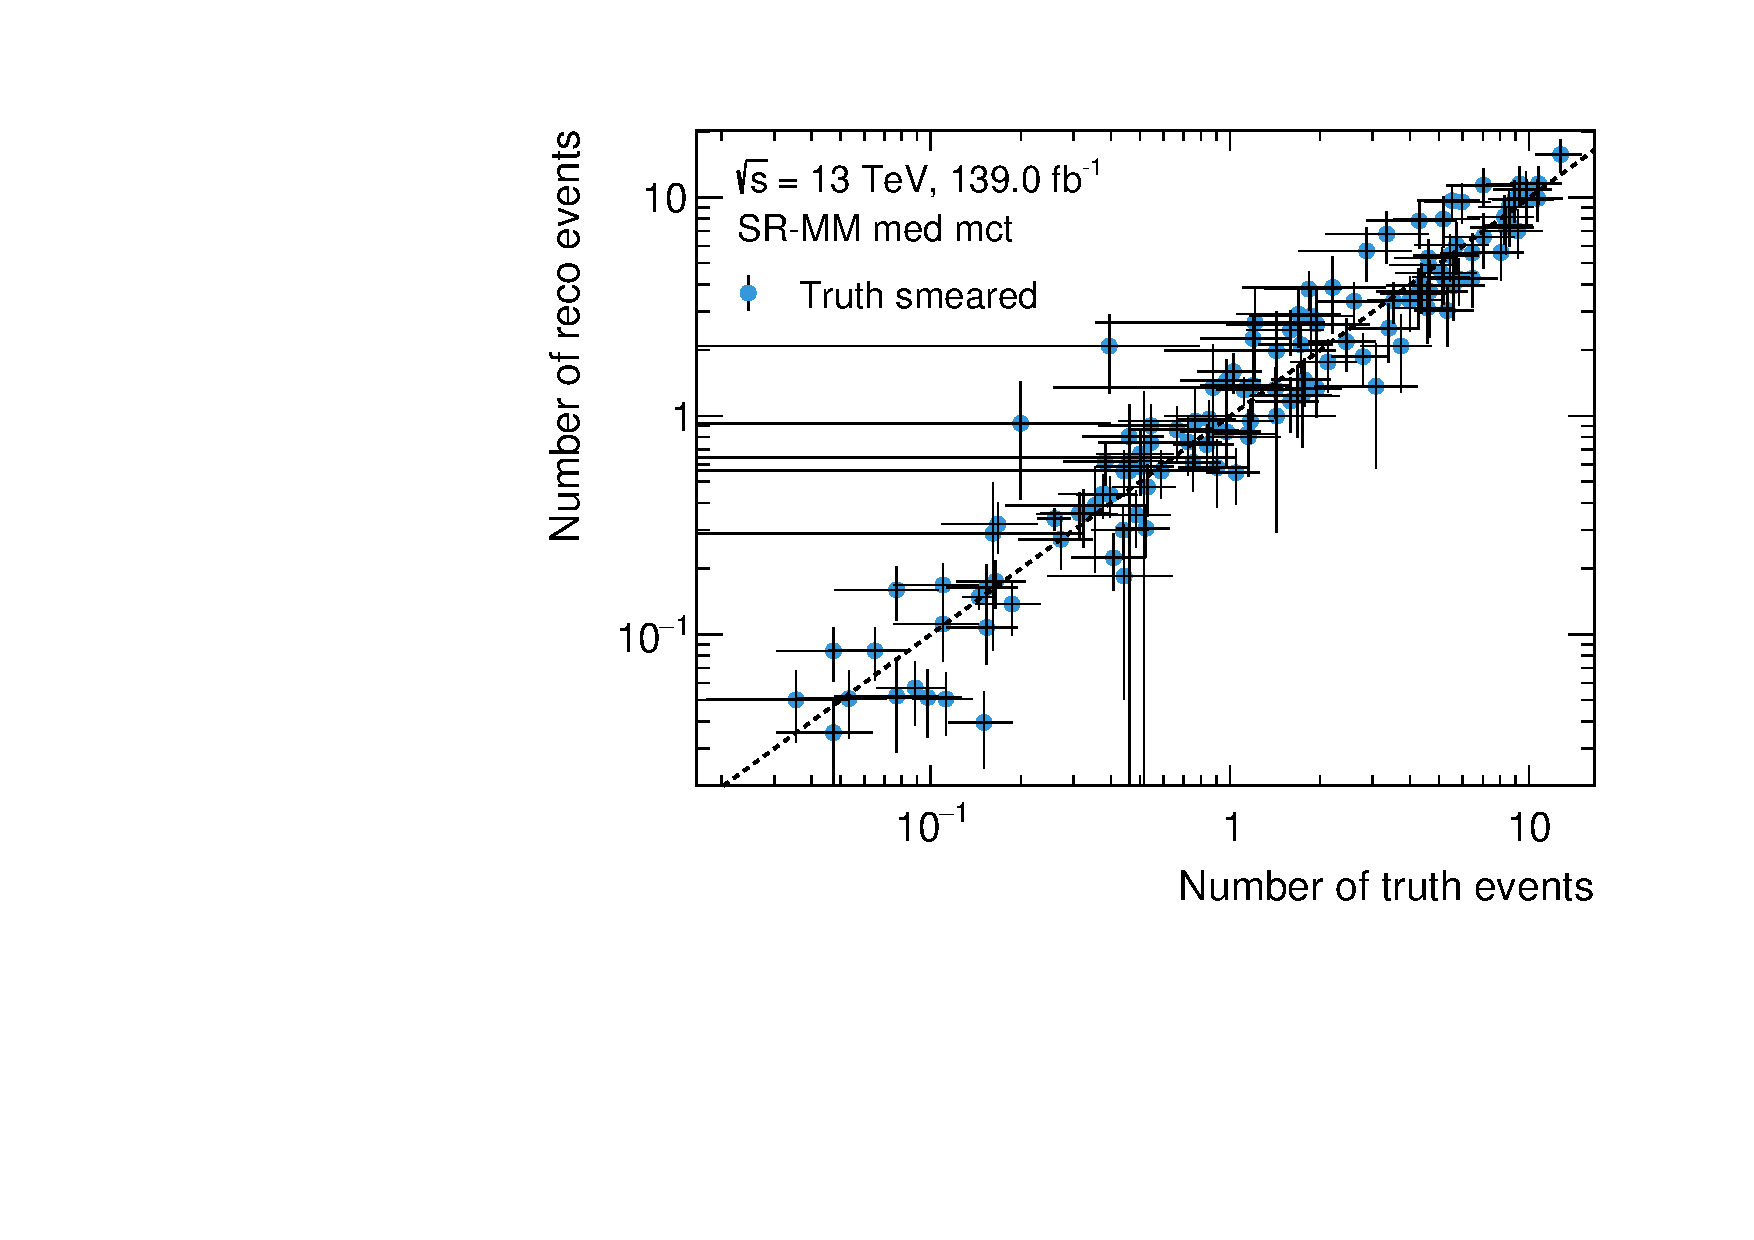
\includegraphics[width=\textwidth]{yields_SR-MM_med_mct_smeared}
	\end{subfigure}\hfill
	\begin{subfigure}[b]{0.49\linewidth}
		\centering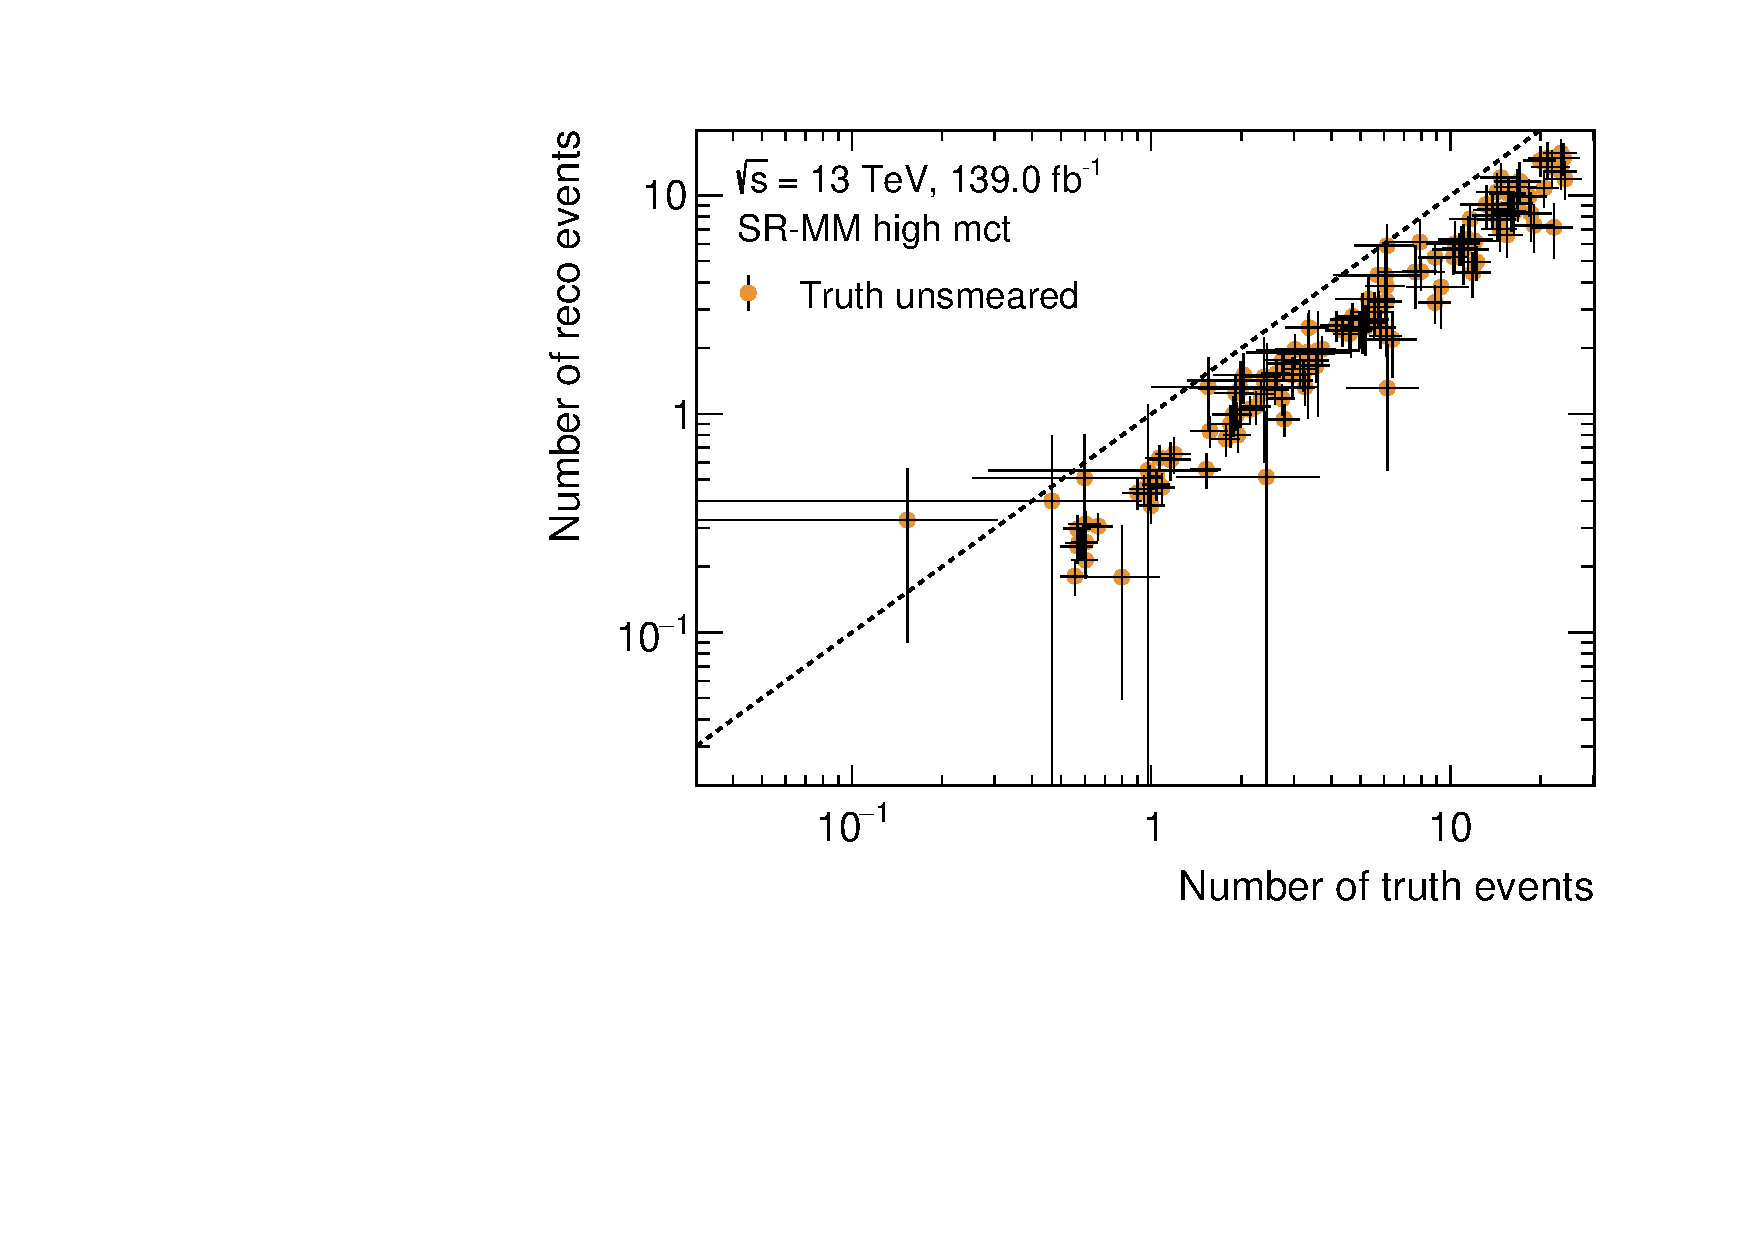
\includegraphics[width=\textwidth]{yields_SR-MM_high_mct_unsmeared}
	\end{subfigure}\hfill
	\begin{subfigure}[b]{0.49\linewidth}
		\centering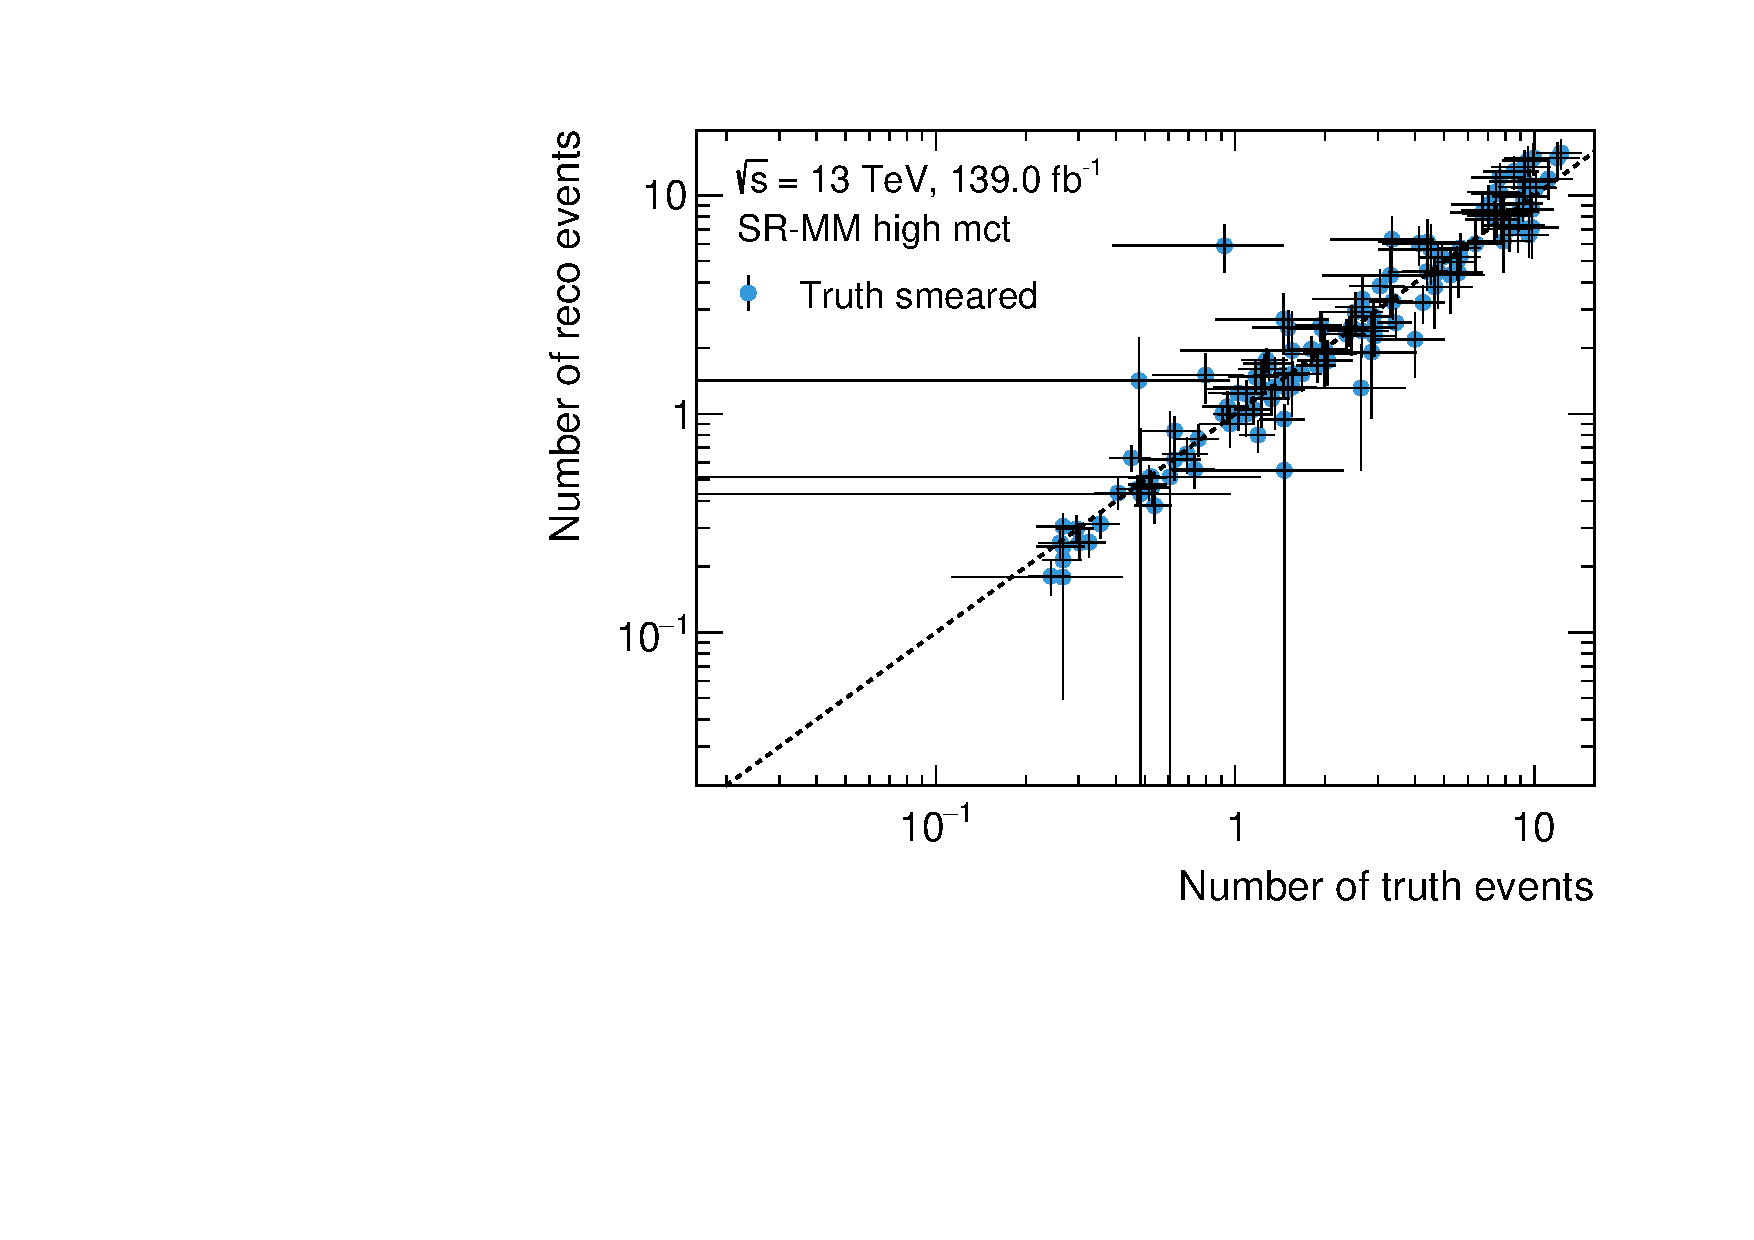
\includegraphics[width=\textwidth]{yields_SR-MM_high_mct_smeared}
	\end{subfigure}
	\caption{Comparison of the event rates at truth- and reconstruction-level before (left) and after (right) truth smearing in SR-MM. From top to bottom, the low, medium and high $\mct$ bins are shown. Every single point in the scatter plots represents a single signal model considered in the original 1-lepton analysis. Uncertainties include only \gls{mc} statistical uncertainties.}
	\label{fig:smearing_signal_regions_2}
\end{figure}

\begin{figure}
	\centering
	\begin{subfigure}[b]{0.49\linewidth}
		\centering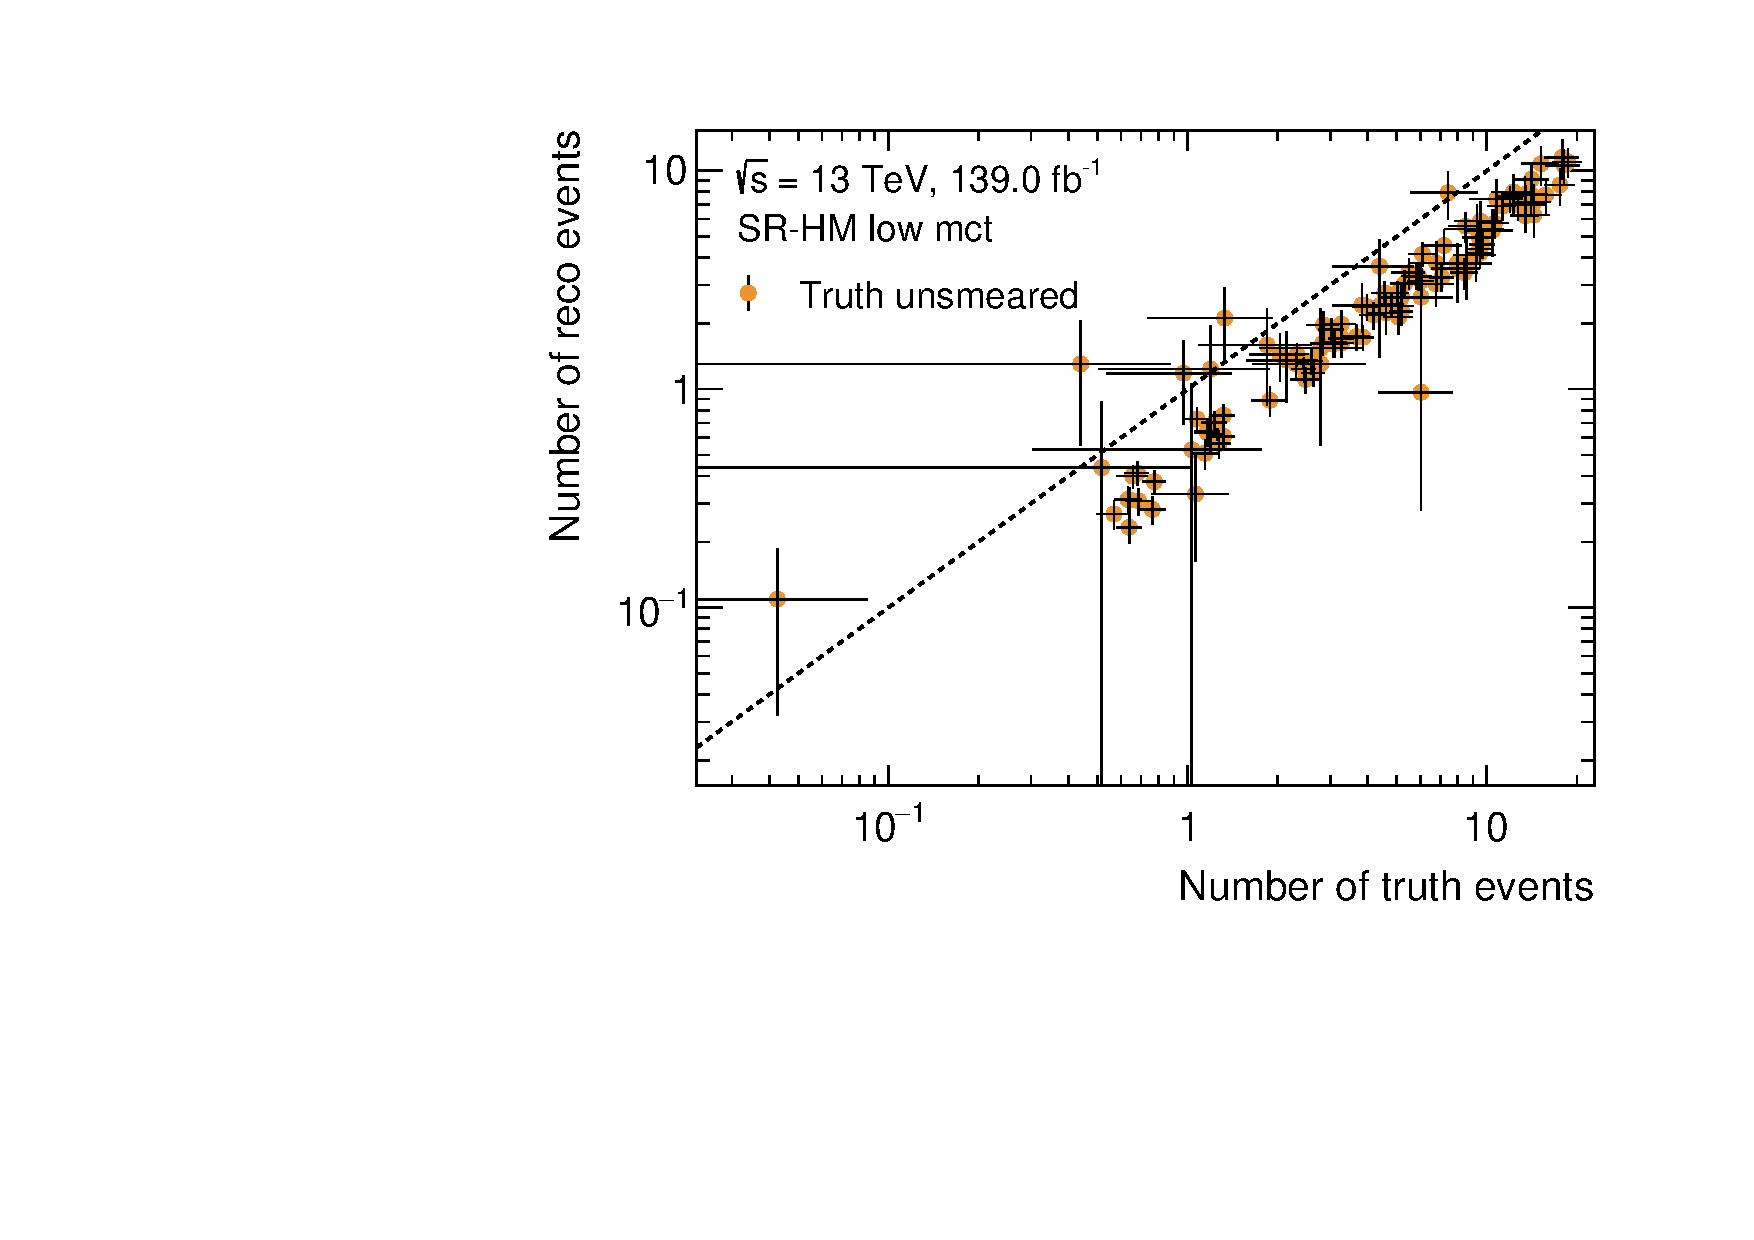
\includegraphics[width=\textwidth]{yields_SR-HM_low_mct_unsmeared}
	\end{subfigure}\hfill
	\begin{subfigure}[b]{0.49\linewidth}
		\centering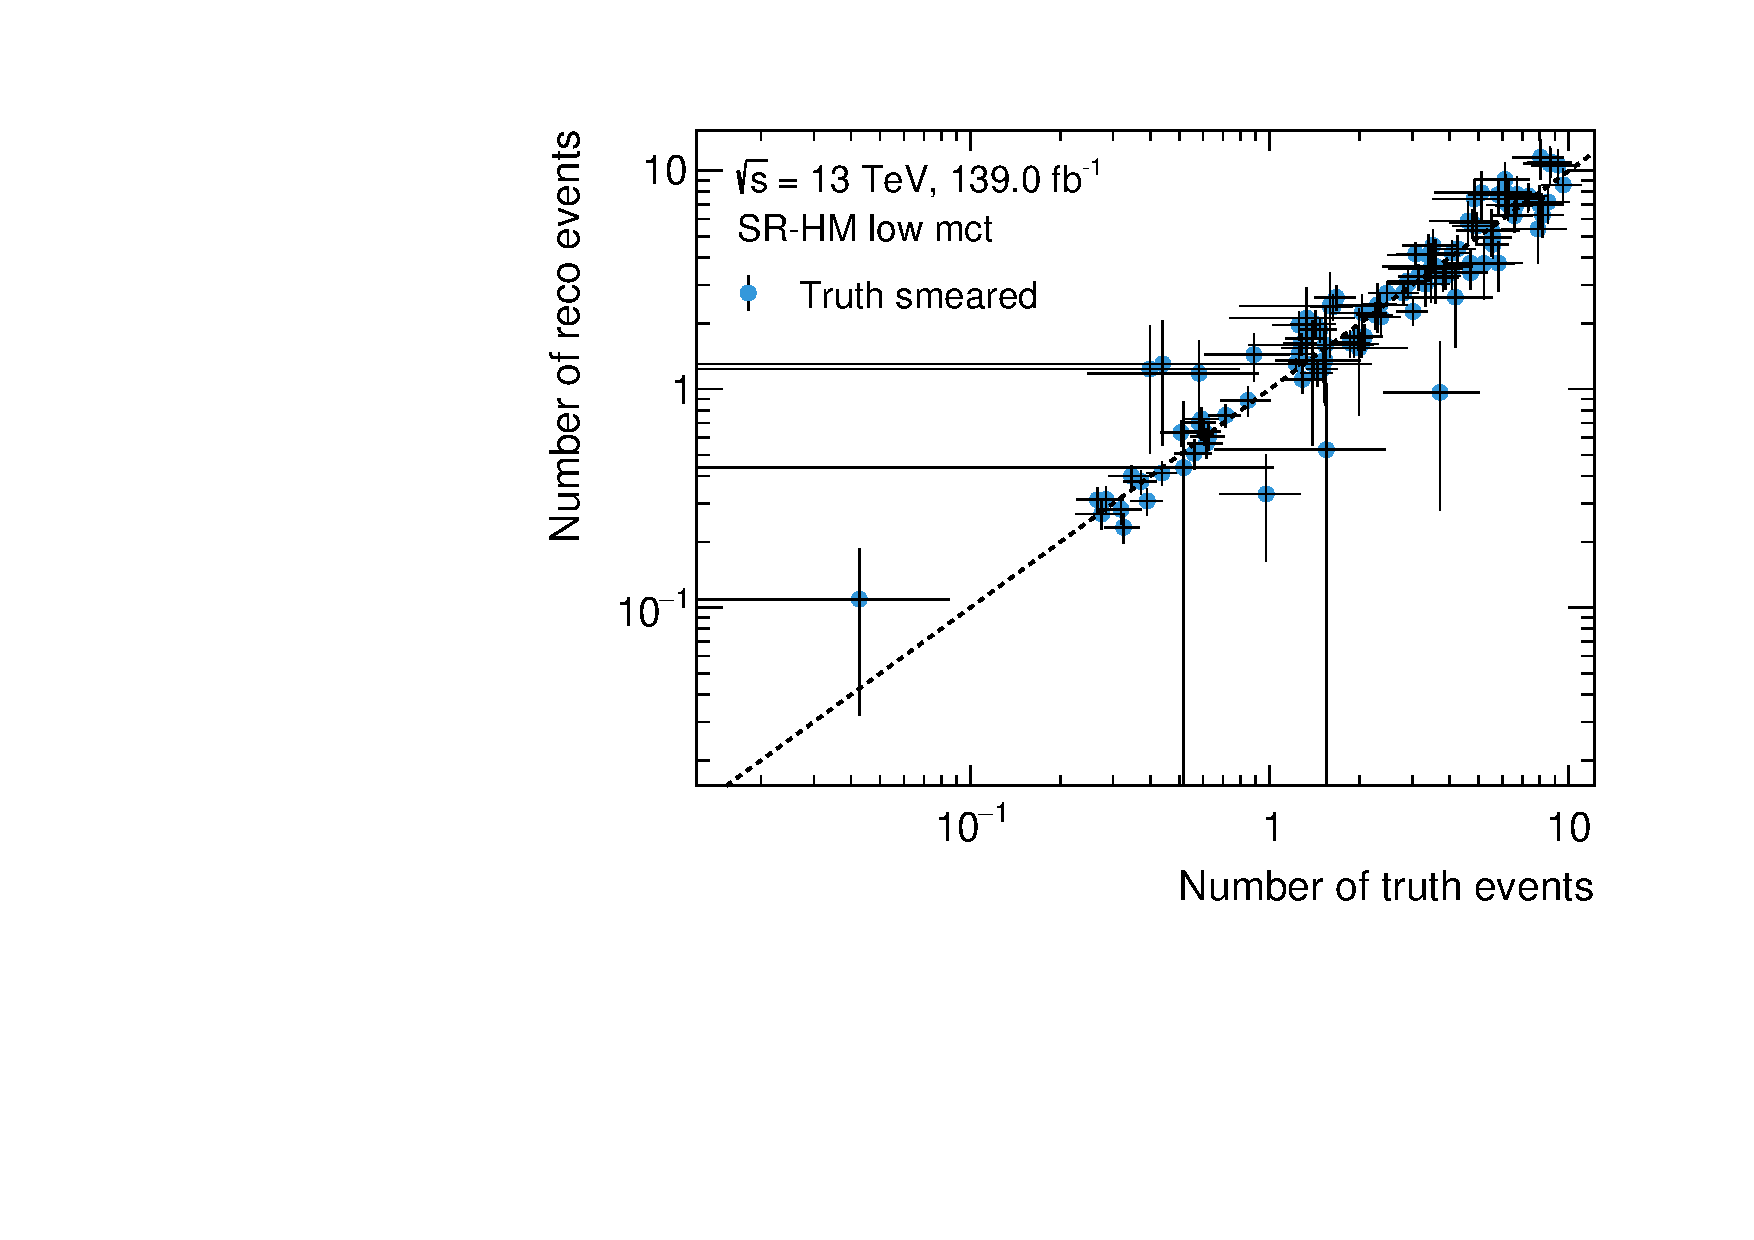
\includegraphics[width=\textwidth]{yields_SR-HM_low_mct_smeared}
	\end{subfigure}\hfill
	\begin{subfigure}[b]{0.49\linewidth}
		\centering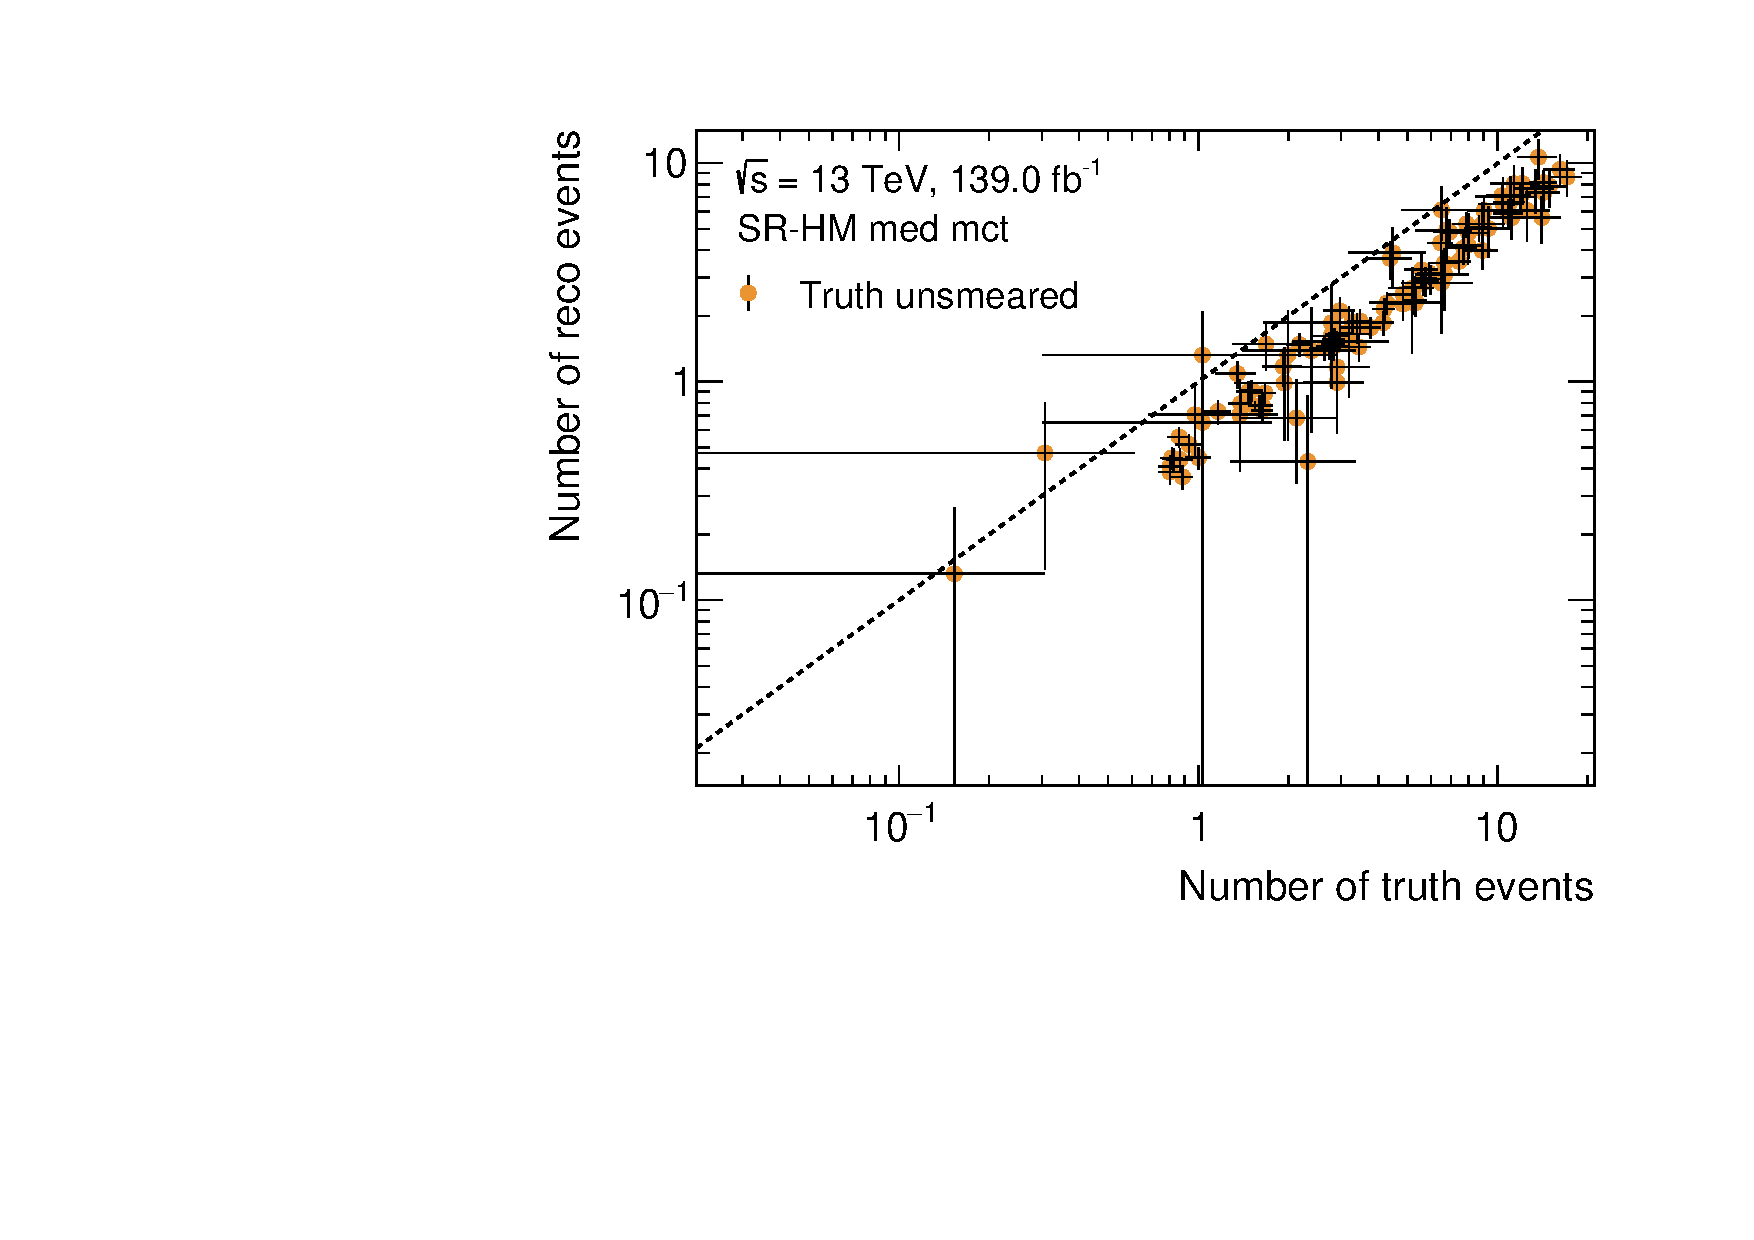
\includegraphics[width=\textwidth]{yields_SR-HM_med_mct_unsmeared}
	\end{subfigure}\hfill
	\begin{subfigure}[b]{0.49\linewidth}
		\centering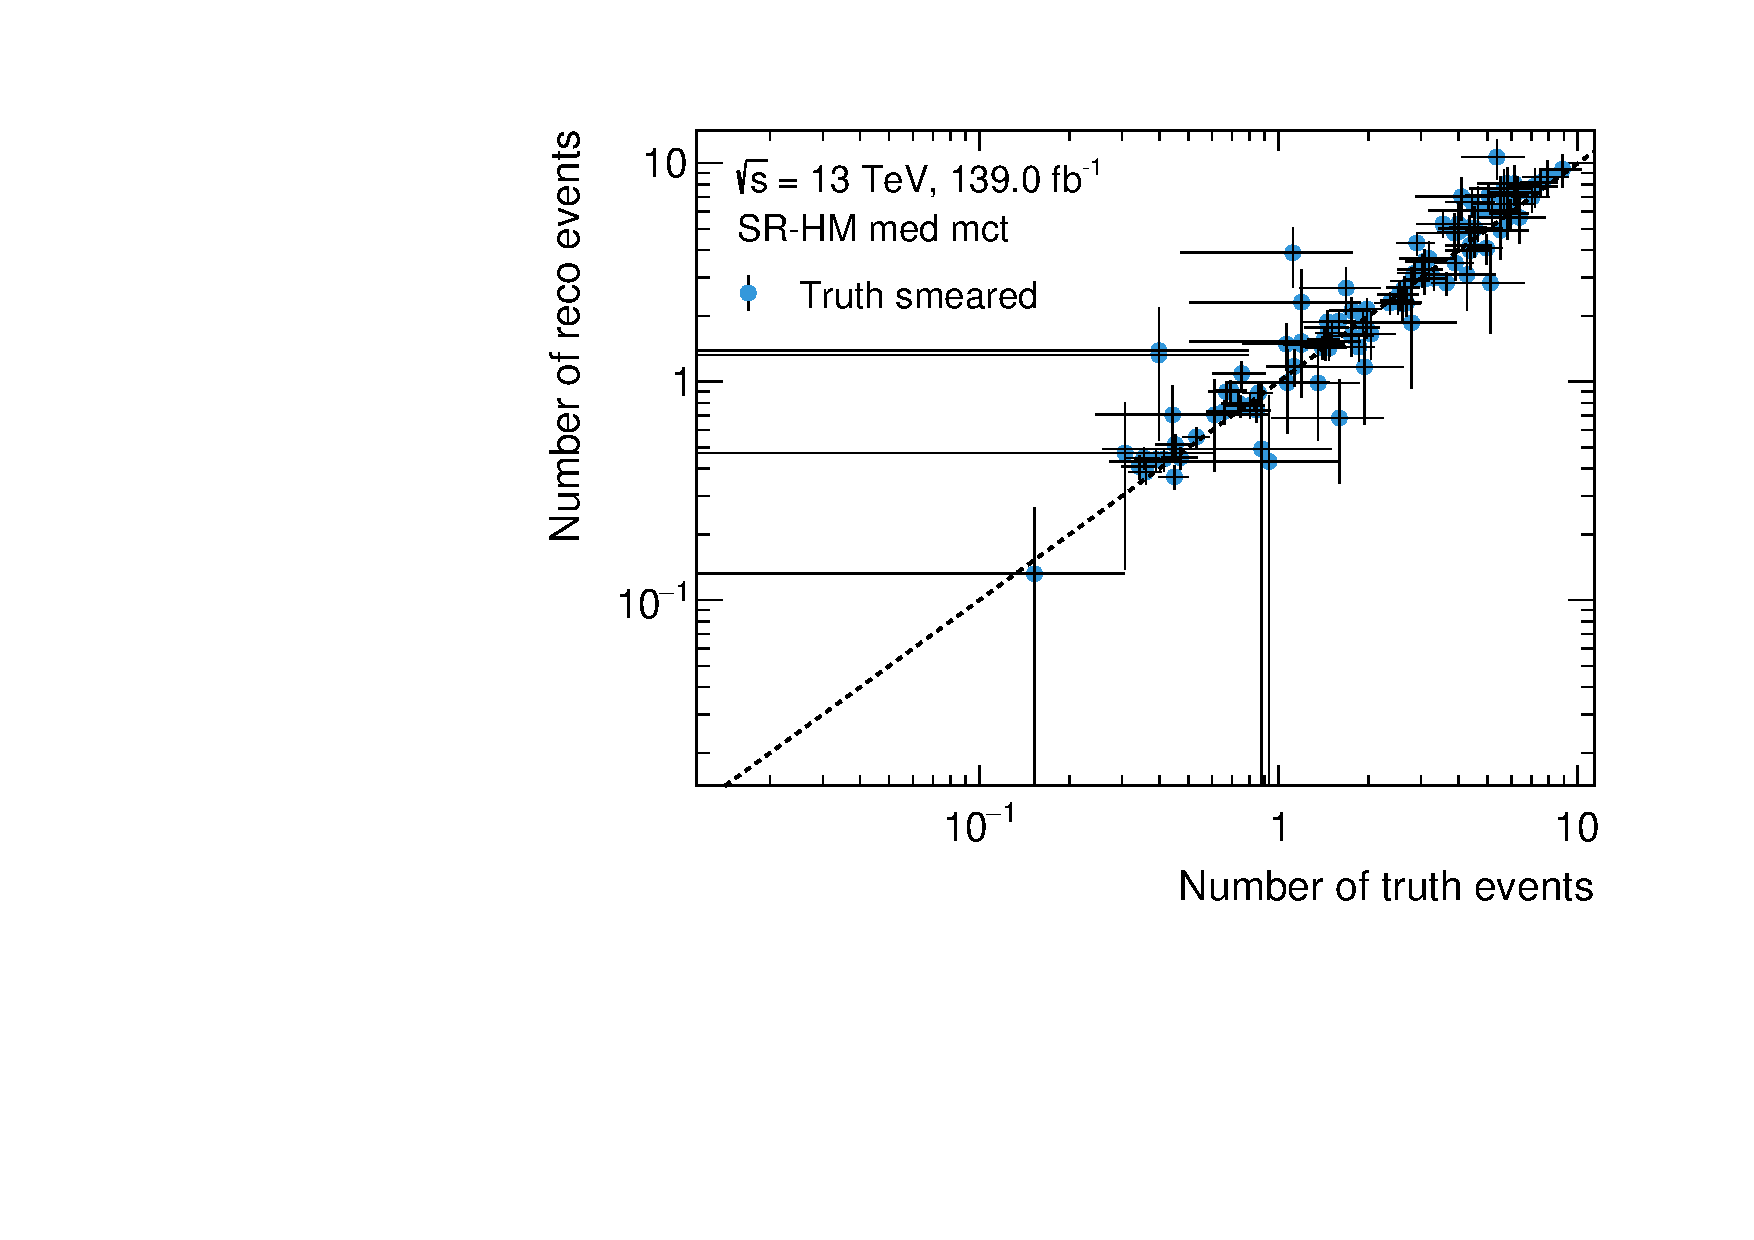
\includegraphics[width=\textwidth]{yields_SR-HM_med_mct_smeared}
	\end{subfigure}\hfill
	\begin{subfigure}[b]{0.49\linewidth}
		\centering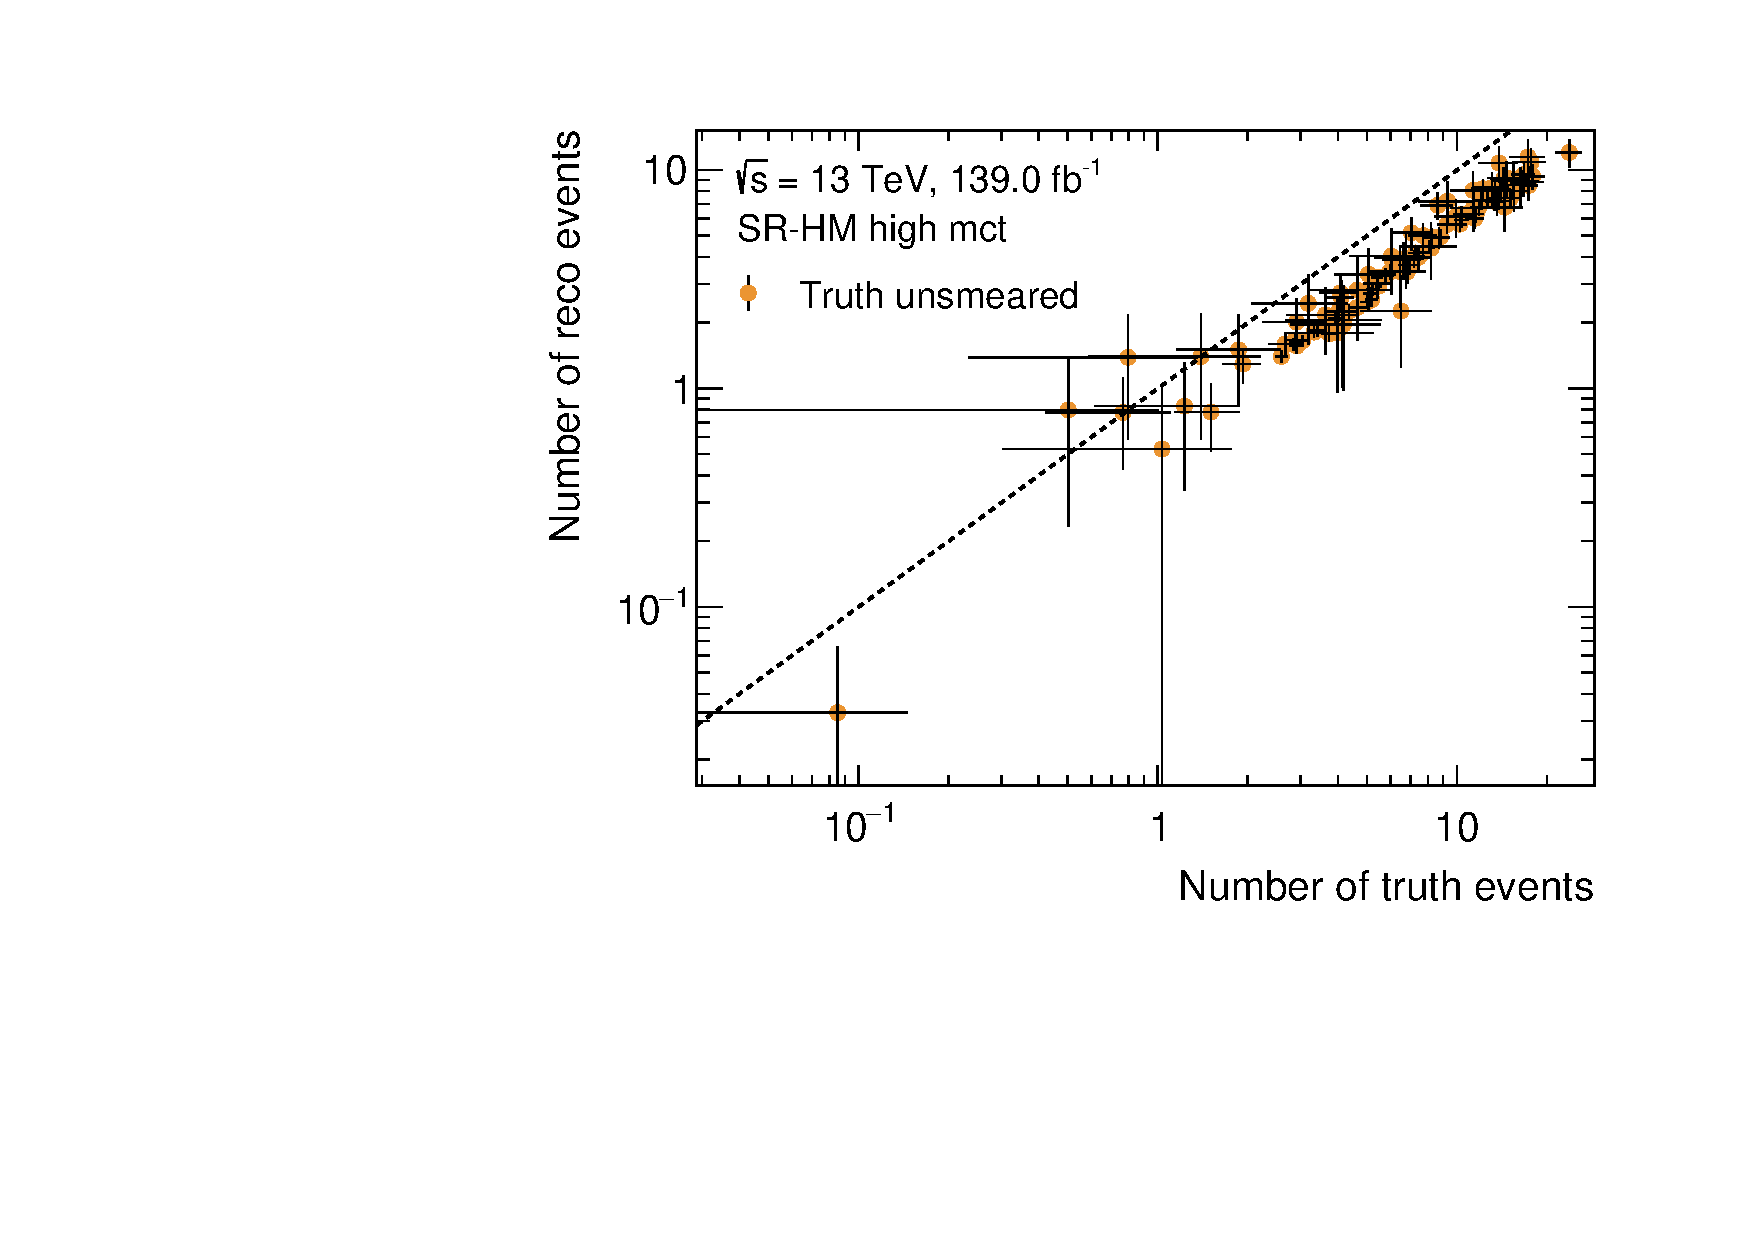
\includegraphics[width=\textwidth]{yields_SR-HM_high_mct_unsmeared}
	\end{subfigure}\hfill
	\begin{subfigure}[b]{0.49\linewidth}
		\centering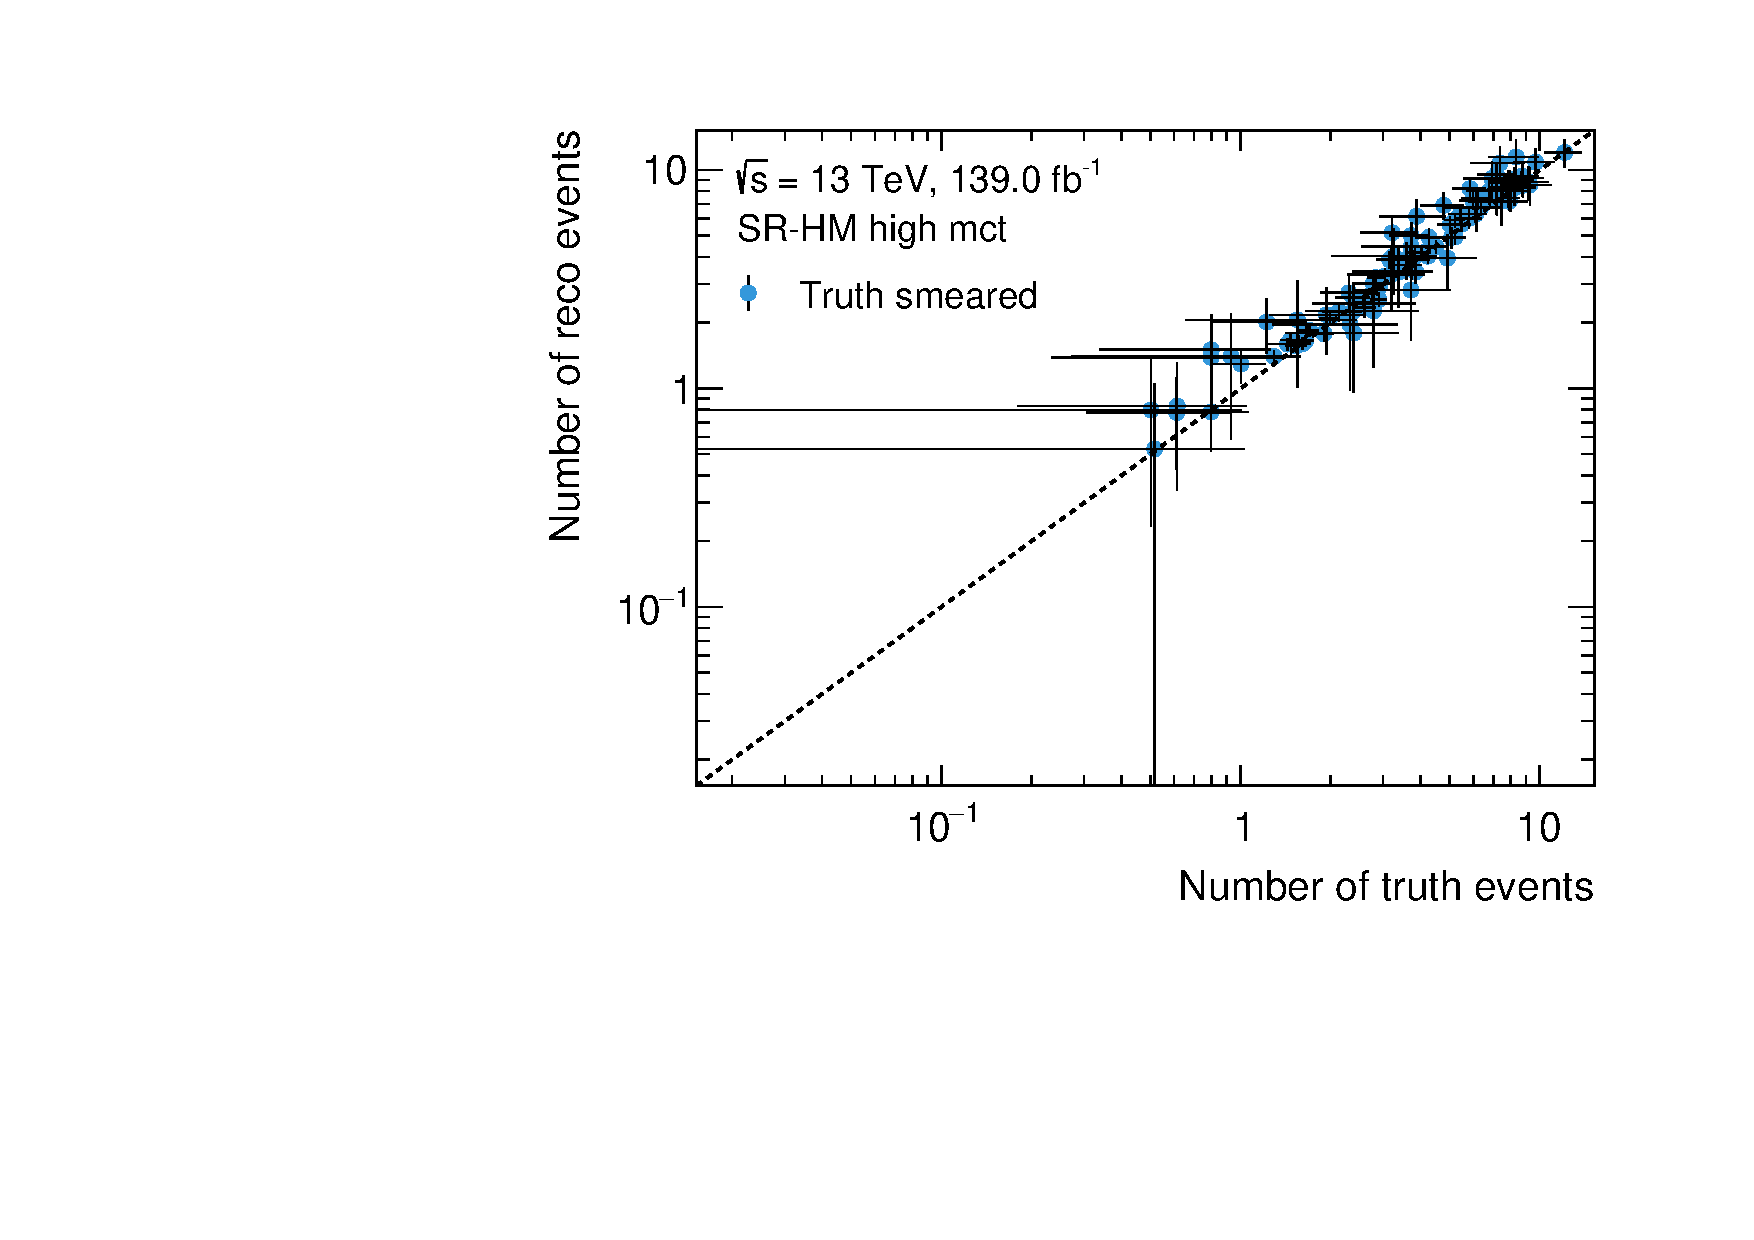
\includegraphics[width=\textwidth]{yields_SR-HM_high_mct_smeared}
	\end{subfigure}
	\caption{Comparison of the event rates at truth- and reconstruction-level before (left) and after (right) truth smearing in SR-HM. From top to bottom, the low, medium and high $\mct$ bins are shown. Every single point in the scatter plots represents a single signal model considered in the original 1-lepton analysis. Uncertainties include only \gls{mc} statistical uncertainties.}
	\label{fig:smearing_signal_regions_3}
\end{figure}
